\documentclass[usletter, 10pt, conference]{ieeeconf} % initial submission to RAL/ICRA
\usepackage{graphicx}
\usepackage{booktabs}
\usepackage{amsfonts}
\usepackage{subfig}
\usepackage[ruled,lined]{algorithm2e}
\usepackage{multirow}
\usepackage{color}
\usepackage{flushend}
\usepackage[bookmarks=false]{hyperref}
\usepackage{setspace} % for setstretch in algorithm
\pdfminorversion=4

\IEEEoverridecommandlockouts                              % This command is only
\overrideIEEEmargins


\newcommand{\red}[1]{\textcolor{red}{#1}}
\newcommand{\tylde}{$\sim$}

%\hypersetup{colorlinks=true,linkcolor=black,citecolor=black}

\SetKwInput{KwData}{Global params.}

\title{Assessing the Accessibility of Protein Tunnels using Motion Planning}

\author{Vojt\v ech Von\' asek$^{1}$,
    Barbora Kozl\'\i kov\'a$^{2}$,
    Adam Jur\v{c}\'\i k$^{2}$,
    Ond\v{r}ej V\'{a}vra$^{3}$,
    Martin Saska$^{1}$
\thanks{$^{1}$ Faculty of Electrical Engineering,  Czech Technical University in Prague, 
Technick\'a 2, 166 27 Prague, Czech Republic, {\tt vonasek@labe.felk.cvut.cz};
$^{2}$ Faculty of Informatics, Masaryk University, Botanick\'a 68a, 602~00 Brno, Czech Republic;
$^{3}$ Loschmidt Laboratories, Department of Experimental Biology RECETOX, Faculty of Science, Masaryk University
    Kamenice 5, 625 00 Brno, Czech Republic. 
The presented work has been supported by the Czech Science Foundation (GA{\v C}R) under research project No. 17-07690S.
}}
%The presented work has been supported by the Czech Science Foundation (GA{\v C}R) under research project No. 17-07690S.
%Access to computing and storage facilities owned by parties and projects contributing to the National Grid Infrastructure MetaCentrum, provided under the programme "Projects of Large Infrastructure for Research, Development, and Innovations" (LM2010005), is greatly appreciated.
%}%
%}
%}



\def\qrand{q_{rand}}
\def\qstart{q_{start}}
\def\qinit{\qstart}
\def\qgoal{q_{goal}}
\def\qnear{q_{near}}
\def\qnew{q_{new}}
\def\T{\mathcal{T}}

\def\C{\mathcal{C}}
\def\CF{\mathcal{C}_{free}}
\def\CFD{{\mathcal{C}^s_{free}}}
\def\dt{d_{tunnel}}
\def\da{d_{atom}}
\def\R{\mathbb{R}}
\def\QI{Q_{init}}
\def\RI{R_{init}}

\def\rv{R_{tunnel}}


\def\Imax{I_{max}} %max number of iterations of RRT-based planners

\def\dist{\mathrm{dist}}
\def\dists{\mathrm{dist}_{\mathrm{s}}}

\SetKw{return}{return}

\def\smin{s_{min}}
\def\smax{s_{max}}
\def\sdelta{s_{\Delta}}


\def\probe{r_{\mathrm{probe}}}
\def\Sprobe{S_{\mathrm{probe}}}

\def\gprobe{r_{\mathrm{out}}}
\def\Sgprobe{S_{\mathrm{out}}}


\def\CG{\mathcal{C}_{goal}}
\def\SB{\mathbf{S}_{blocking}}
\def\SS{\mathbf{S}}


%spacing for algorithm environment. 1.0 mean normal spacing
\def\gb{p_{tunnel}}

\def\L{\mathcal{L}}
\def\S{\mathcal{S}}

\def\LA{L_1}
\def\LB{L_2}

\def\RA{A$_{1}$}
\def\RB{A$_{2}$}
\def\RC{A$_{1}^{*}$}
\def\RD{A$_1^P$}


% ==================================================================================

\begin{document}

\maketitle
\thispagestyle{empty}
\pagestyle{empty}

\begin{abstract}
Chemical interactions between proteins and other molecules (ligands) take place in specific locations, called active sites, that are often deeply buried inside the protein structure.
These active sites are accessible through one or more void paths, called tunnels.
Nowadays, tunnels are mostly computed using Voronoi diagrams which approximate the ligand by a bounding sphere.
This leads to highly imprecise results.
To address this problem, we define the computation of the transportation path of non-spherical ligands including their conformation changes (i.e., when the atoms of the ligand move relatively to each other) as a motion planning task in high-dimensional configuration space.
This can be solved using sampling-based planning methods.
We propose a modification of the Rapidly Exploring Random Tree planner for the purpose of trajectory computations of flexible ligands.
To cope with the narrow passage problem, the random samples are generated around a Voronoi-based tunnel.
%which serves us for better localization of the searched space.
The flexibility of the ligand is modeled using a fixed set of known conformations, which does not increase the number of dimensions of the configuration space.
The proposed method has been evaluated in a virtual screening scenario to estimate the traversability of tunnels for several ligands.
\end{abstract}


\section{Introduction \& Motivation}


Reactivity of proteins with other molecules plays a crucial role in many research disciplines, including protein engineering and drug design.
Protein reactivity is tightly connected with the presence of the void space between its amino acids. 
This space, forming a path called tunnel, can be utilized by a small molecule (ligand) which can enter the protein inner space and react with its amino acids surrounding a specific site, called the active site~\cite{gora2013gates}.
\textcolor{blue}{The size and location of tunnels determine the ligand size and shape which can enter the active site.}
Currently, the biochemists use various computational methods for tunnel detection (Fig.~\ref{fig::motiv}) in order to estimate the possibility of interactions between a protein and a ligand.
This helps them to reduce the number of necessary in-vitro lab experiments.
The most common tools detect the tunnels using Voronoi diagrams~\cite{yaffe2008,caver3} assuming a spherical ligand (probe), 
i.e., they approximate the ligand by a bounding sphere.
However, the ligands are typically of a non-spherical shape which is completely ignored by these methods. 


\begin{figure}[t]
\centering
{\footnotesize
\renewcommand{\arraystretch}{-0.5}
\renewcommand{\tabcolsep}{-1pt}
\begin{tabular}{ccc}
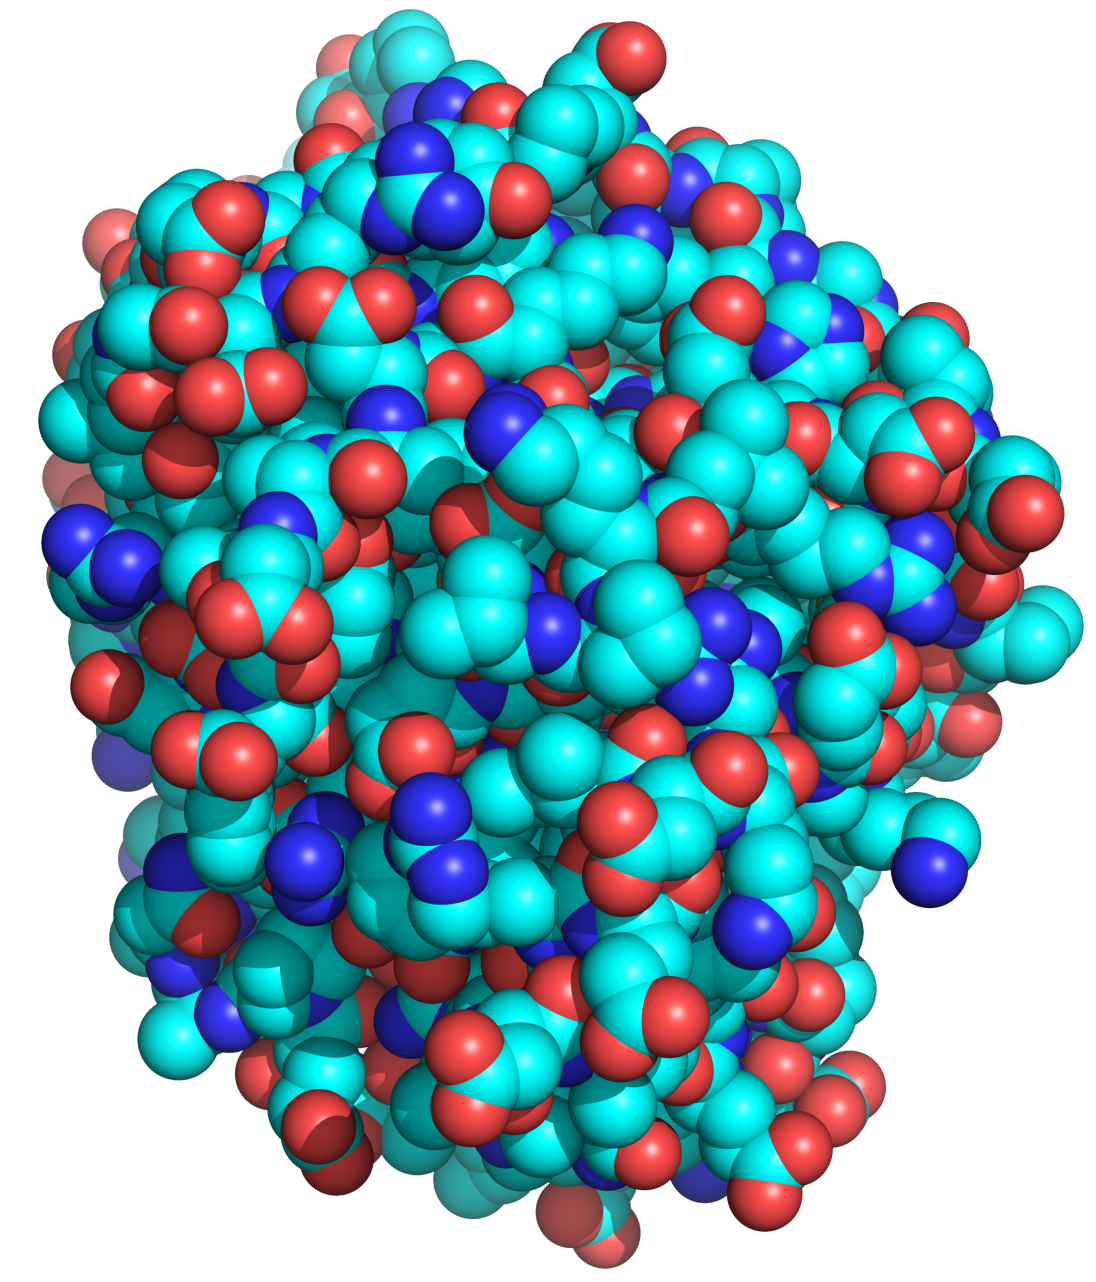
\includegraphics[width=0.14\textwidth]{fig/motiv1} &
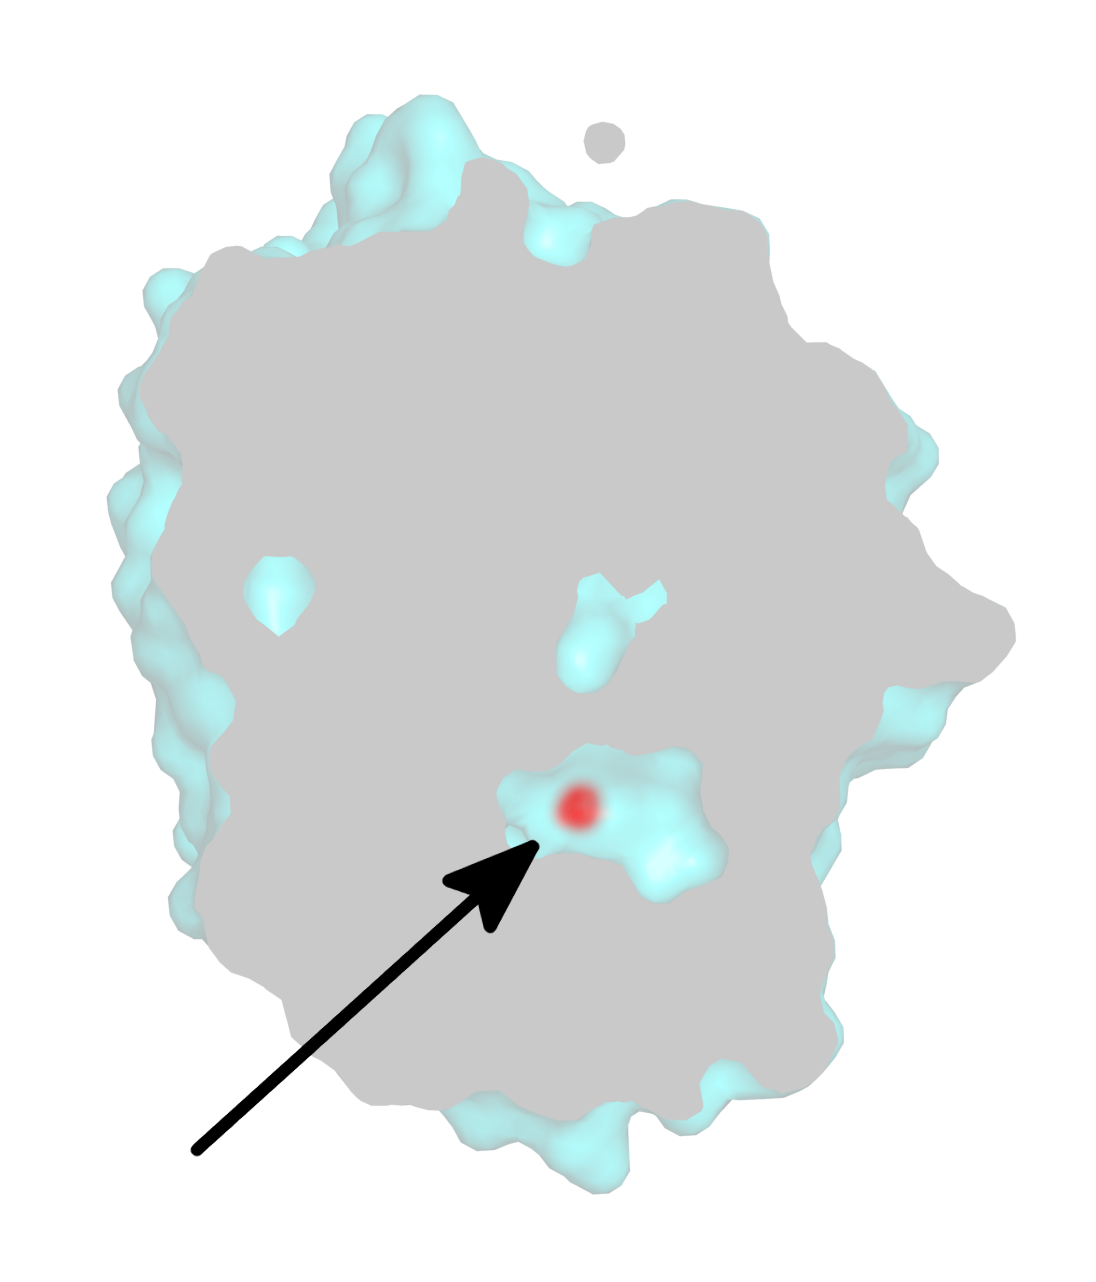
\includegraphics[width=0.15\textwidth]{fig/motiv2lab} &
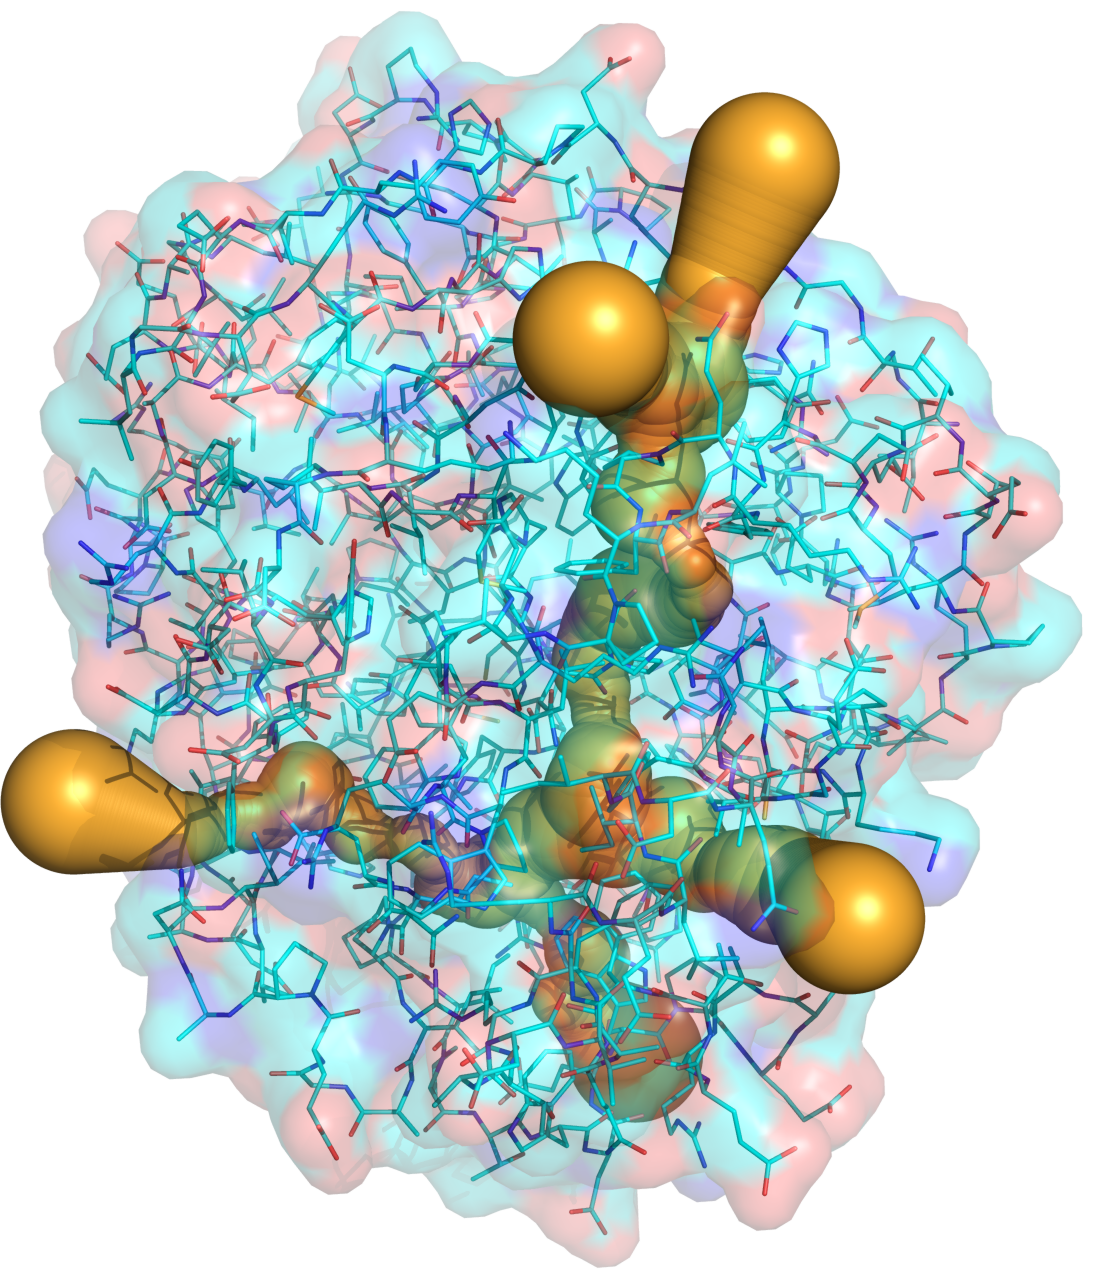
\includegraphics[width=0.14\textwidth]{fig/motiv3}  \\
Protein  & Active site & Detected tunnels \\ %& Example of a  \\
             &            & (orange)         \\  %& trajectory
\multicolumn{3}{c}{%
\includegraphics[width=0.16\textwidth]{fig/renderDCP}  \hskip 15pt
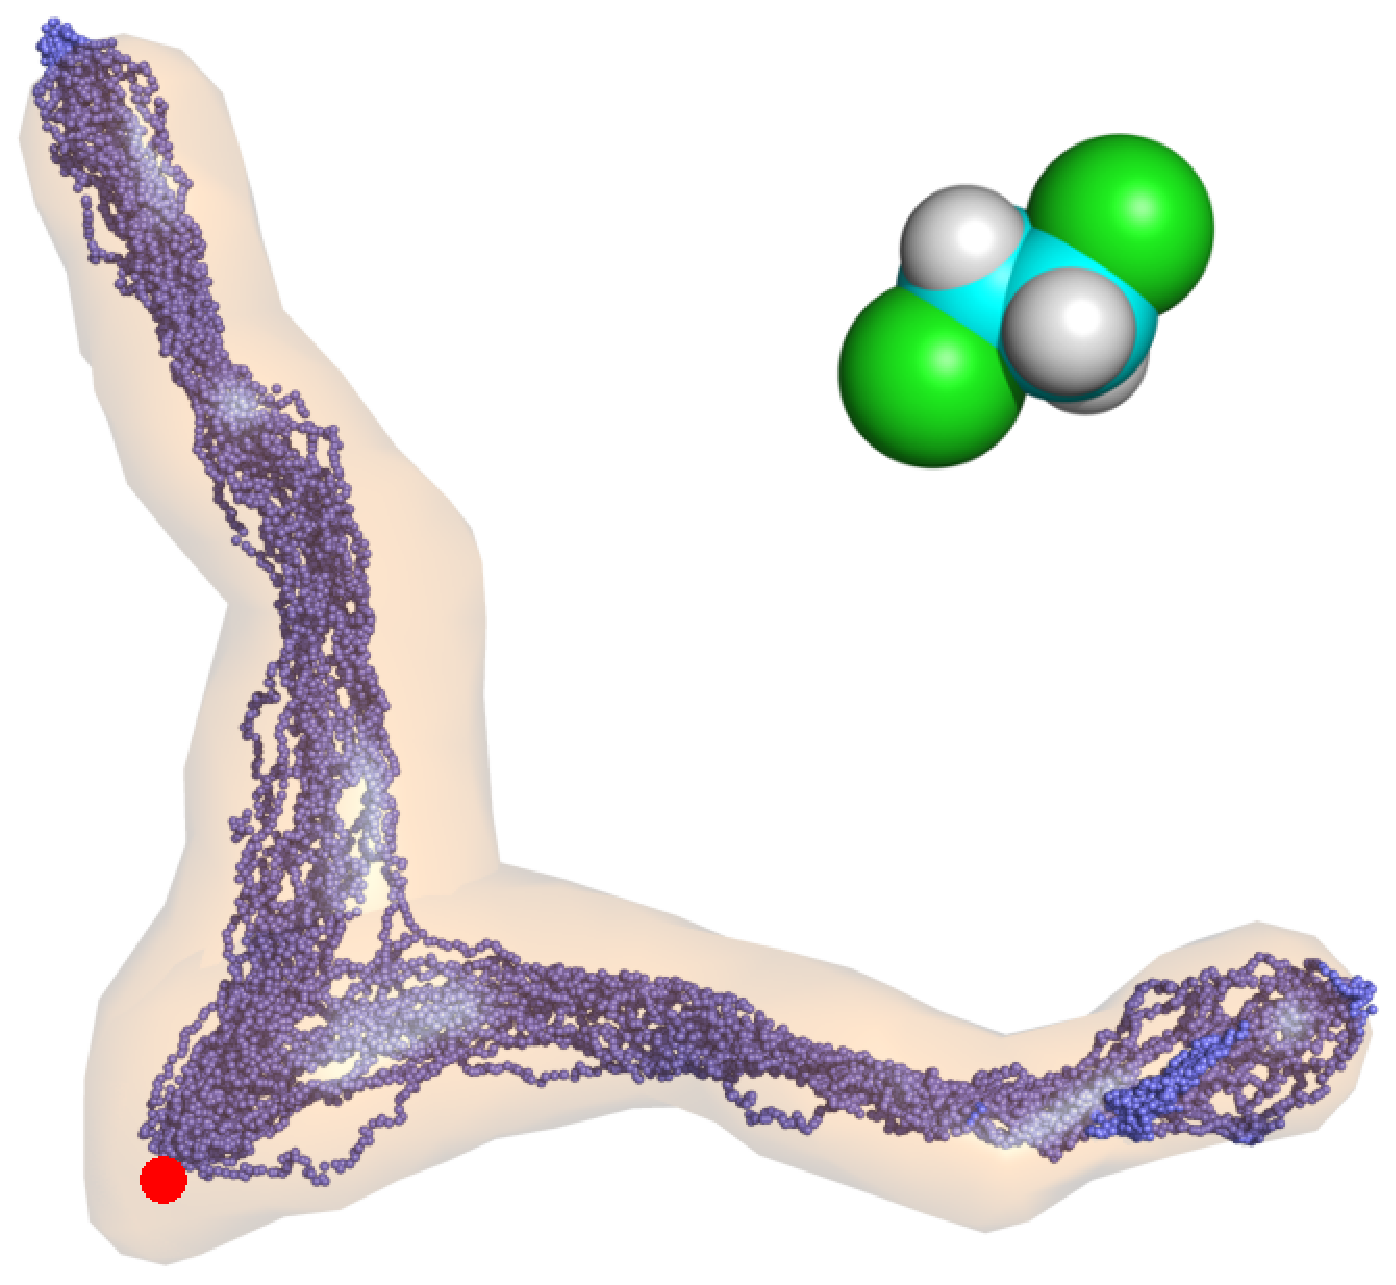
\includegraphics[width=0.14\textwidth]{fig/render37t}} \\ 
\end{tabular}
}
\caption{\label{fig::motiv}
    \small
    Tunnels in the Haloalkane dehalogenase protein with possible trajectories of 1-Chlorpropan ligand (bottom left) and 1,2-Dichloroethane (bottom right).
}
\end{figure}

Our approach aims to overcome this problem by taking into account the actual shape of the ligand.
This necessarily requires to consider also conformational changes, i.e., the mutual position of the ligand atoms can change.
Such a ligand is denoted as flexible ligand.
%Our approach aims to overcome this problem by taking into account the actual shape of the ligand and also its conformations.
%\textcolor{blue}{To provide the biochemists with a solution which detects tunnels also in these frames and understand the ligand passage, it is necessary to take into account not only the ligand shape but also its conformation changes when the ligand moves.}
%The proposed solution needs also to cope with the narrow passage problem, as proteins are dense structures limiting the ligand movements inside.
%Such a ligand, for which the mutual position of its atoms can change, is denoted as a flexible ligand.

The analysis of traversability of the tunnels by flexible ligands can be formulated as a motion planning problem and
solved by sampling-based planners.
Sampling-based planners randomly sample the configuration space of the robot (ligand) and connect the collision-free samples
into a graph structure (roadmap).
Rapidly Exploring Random Tree (RRT)~\cite{lavalleRRT} is one of the most used sampling-based planners.
Besides many applications in robotics, the sampling-based planners have been already used in biochemistry as well, 
e.g., to study loop motions~\cite{cortes2004geometric}, to identify binding sites~\cite{bayazit2001ligand}, for exit
pathway detection~\cite{cortes2010simulating,cortes2005path} and especially for protein folding~\cite{raveh2009rapid,amato2002using}. %novinskaya2015improving

%Sampling-based planners can cope with many-DOF systems and they have been successfully employed also beoynd robotics, e.g. to
%identify binding sites~\cite{bayazit2001ligand} or to determine ligand exit pathway~\cite{cortes2010simulating}.
%The random samples are classified as free or non-free using black-box collision detection which allows the sampling-based methods to find paths for robots of various shapes. 
%The sampling-based planners can cope with robots with many degrees of freedom (DOF).
%Two most commonly used sampling-based techniques are Probabilistic Roadmaps (PRM)~\cite{kavrakiForPP} and Rapidly Exploring Random Trees (RRT)~\cite{lavalleRRT}.
%Therefore, they have been used for motion planning of various robotic systems.
%Sampling-based motion planners has been intensively studied in robotics, but they have been applied also in other research fields.
%In bio-chemistry, the planners have been used to study
%protein folding~\cite{amato2002using,raveh2009rapid,novinskaya2015improving,songPFintro},
%or for tunnel detection~\cite{vonasek2017tunnel}.

In this paper, we propose a modification of the RRT planner to find trajectories for non-spherical flexible ligands inside protein tunnels.
The random samples are generated around a given tunnel instead in the whole configuration space.
%We localize the generation of the random samples, i.e., instead of sampling the whole configuration space we focus only on the space surrounding a potential tunnel detected by the Voronoi-based method (using a smaller ligand probe in order to avoid omitting possibly feasible tunnel candidates).
The potential tunnel is represented by a set of consecutive spheres surrounding the tunnel centerline.
To enable the movement of the ligand in the narrow parts of the tunnel, the free-space is dilated by shrinking the atom radii, similarly, e.g., to~\cite{hsu06multilevel}.  %cortes2005path removed as it is not clear it they really rescale
The ligand flexibility is modeled using a fixed set of predefined conformations which the ligand can occupy.

Finding trajectories only along a given tunnel tunnel is faster than computing any exit pathway from the protein due to decreased
volume of the configuration space to be searched.
Another advantage of our method in comparison with the existing approaches is that we enable the users to trace the ligand path leading from the
\textcolor{blue}{outside/outer?} solvent towards the protein active site.

The proposed method was tested by the biochemists who compared the results with already known trajectories of ligands, determined by their traditional approaches.
In the following section, we first mention several approaches and methods related to our solution and then we describe the proposed method in detail.

\section{Related Work}

Most of the available tools for tunnel detection are based on Voronoi diagrams~\cite{yaffe2008,caver3} or they utilize a grid-based computation~\cite{sehnal2013mole}.
%The tunnels are pathways computed for a single atom (spherical probe) using Voronio-diagrams~\cite{yaffe2008,caver3} or 
%grid-based approaches~\cite{sehnal2013mole,petrek2006caver}.
The tunnels are represented as a sequence of spheres and characterized by their bottleneck, length, curvature, and a list of surrounding residues, whose physico-chemical properties are crucial for assessing the interaction possibilities between the protein and ligand.
More details can be found in the recently published state-of-the-art report about analysis and visualization of biomolecular cavities~\cite{Krone_2016}.
The main disadvantage of both grid-based and VD-based methods is that the shape of the ligand is not taken into account during the tunnel detection and it is therefore not easy to estimate if (and how) a non-spherical ligand can traverse the tunnel.
The ligand flexibility cannot be principally considered by these approaches.
Simulations based on molecular dynamics (MD) can directly evaluate the migration of a ligand into a protein, but they are significantly more computationally demanding~\cite{kingsley2014including}. 
Moreover, MD simulations have to be prepared for a specific ligand/protein pair, which is not practical for testing a large number of ligands.
The geometric-based methods are therefore still preferable due to their speed.

The traversability of a tunnel by a flexible ligand can be formulated as a motion planning problem and solved using sampling-based motion planners.
These planners can cope with objects (robots) with many Degrees of Freedom (DOF)  and they can also consider objects of arbitrary shape.
Two widely used planners are Probabilistic Roadmaps (PRM)~\cite{kavrakiForPP} and Rapidly Exploring Random Tree (RRT)~\cite{lavalleRRT}.
%Sampling-based planners like RRT can be used to find the trajectories even for flexible ligands, as they can cope with many-DOF systems and they can consider arbitrary shape.
%The computation of the ligand trajectories can be solved also using motion 
%In order to determine if the ligand can pass the tunnel using the geometric-based methods, it is necessary to compute a trajectory considering the shape of the ligand and its 3D translation and rotation.
%In each iteration of RRT, a random configuration $\qrand \in \C$ is generated and its nearest node $\qnear \in \T$ in the tree is found.
%A new configuration $\qnew$ is constructed on the line connecting $\qnear$ and $\qrand$ in the distance $\varepsilon$ from $\qnear$.
%If $\qnew$ is collision-free, it is added to the tree.
%The algorithm terminates if the tree approaches the goal configuration close enough.
%rrt for molecular: \cite{al2012motion}
%survey \cite{gipson2012computational}
%Solutions for tunnel detection using sampling-based methods however have not been discussed yet.
%Sampling-based planners have been used in various applications in robotics~\cite{elbanhawi2014sampling} and also  %,latombe1999motion} and also
% to study proteins, e.g. in  
%loop motions~\cite{cortes2004geometric},
%protein folding~\cite{amato2002using,raveh2009rapid,novinskaya2015improving,songPFintro},
%protein folding~\cite{raveh2009rapid,novinskaya2015improving},
%or protein folding combined with ligand diffusion~\cite{cortes2010simulating}.
The well known issue of the sampling-based planners is the narrow passage problem.
Narrow passage is a small region in the configuration space, whose removal changes the connectivity of the space.
Due to its low volume, the probability of sampling the narrow passage is low.
Consequently, many iterations are needed in order to put enough samples into the passages, which increases the computation time.
PRM-based planners can cope with the narrow passage problem by increasing the probability of sampling in difficult regions, e.g.
by sampling along medial axis~\cite{amatoOBRRT,amato2002using,wilmarthMAPRM}.
In~\cite{bergWIG}, workspace is represented by a grid in which difficult regions are identified using watershed labeling.
The regions can be estimated online, e.g., based on the number of collision-free samples around a given configuration~\cite{overmarsGauss,hsuBridge} or even identified by a human operator~\cite{denny2018general}. 
%The narrow passages are however located in the configuration space and it is generally not easy to estimate their location
%based only on the features of the workspace~\cite{hannaWIS}.
%.g. based on amount of collision-free samples around a given sample~\cite{overmarsGauss} or e.g. based
%~\cite{hsuBridge,overmarsGauss}.

%In the Gaussian sampling strategy~\cite{overmarsGauss}, the samples are generated more frequently around obstacles.
%A random configuration $q_1\in\C$ is generated uniformly and another random configuration
%$q_2\in\C$ is drawn around using Normal distribution $N(q_1,\sigma^2)$.
%If both $q_1$ and $q_2$ are free or both are non-free, they are not added to the roadmap. 
%If only one of these configurations is free, then the free one is added to the roadmap. 
%The disadvantage of this strategy is the necessity to choose suitable value of the parameter $\sigma^2$, which depends
%on the used map and the shape of the robot.
%The Bridge-Test sampling~\cite{hsuBridge} employs the Gaussian strategy to generate two samples in order to compute their midpoint.
%The Gaussian strategy was improved in the Bridge-Test~\cite{hsuBridge}. % to generate samples inside a narrow passage.
%Two random configurations $q,q'\in\C$ are generated in same way as in the Gaussian strategy.
%The midpoint $p$ on a segment $q,q'$ is constructed.
%If the midpoint is collision-free and both end configurations are non-free, the midpoint lies in a narrow passage, and it is added to the roadmap.
%Both Gaussian and Bridge-Test strategies have to be combined with the uniform sampling in order to ensure sampling of free-regions~\cite{sun2005narrow}.
%Despite the simplicity of these two modifications, they were proven to significantly improve performance of PRM~\cite{hsuOnProb,geraertsRA,geraertsPRMA,wang10adaptive}.

RRT-based planners cannot cope with the narrow passage problem simply by increasing the probability of sampling in the difficult regions, as the
growth of the configuration tree towards the random samples may be blocked by obstacles. %~\cite{vonasekphd}.
To prevent this blocking, DD-RRT~\cite{yershovaDDRRT} limits the selection of nodes for expansion to a small ball. 
The radius of the ball is set to infinity for new nodes, and decreases to a predefined radius if the node cannot be successfully expanded.
Automatic adaptation of this radius was proposed in ADD-RRT~\cite{jailletADRRT}.
%The disadvantage of DD-RRT is the sensitivity to the predefined radius.
%Therefore, the authors of ADD-RRT~\cite{jailletADRRT} proposed to adapt the ball radius according to the success rate of the expansion.
To attract the tree towards a given region, random samples have to be generated there only if the tree can expand to this region.
In~\cite{kardossRRTKK}, the probability of sampling is increased in several waypoints close to narrow passages, but without specifying
how to find these waypoints.
The generalization of~\cite{kardossRRTKK} is the guided sampling, where a whole path is used
to generate samples in the configuration space.
The path can be computed in the workspace~\cite{vonasek2009rrt}, or iteratively refined in the configuration space based on the solution of a relaxed version of the problem~\cite{bayazitIRC}.

%~\cite{vonasek2009rrt,denny2016dynamic,denny2014marrt}.
%This is the main idea of the guided sampling~\cite{vonasek2009rrt,denny2014marrt,denny2016dynamic}, where a the configurations

%Another techniques to sample the narrow passages dense enough is to retract the random samples towards regions that are believed
%to be located in narrow passages~\cite{zhangRetraction,lee2012srrrt}.
%the random sample $\qrand$ is connected to the tree if the line segment  from $\qnear$ to $\qrand$ is collision-free. Otherwise, the retraction-step is performed.
%The task of the retraction step is to find a contact configuration around $\qnear$ that minimizes the distance to $\qrand$.
In Retraction-based RRT~\cite{zhangRetraction}, the tree is retracted along the boundary of the obstacles in the configuration space.
This requires the analysis of the contact space, which leads to the generalized penetration depth computation of high complexity~\cite{he2016efficient}. %\cite{he2016efficient} in RAL!! + zhang2008fast
Selective Retraction-based RRT~\cite{lee2012srrrt} avoids the expensive growth in the open areas of the configuration space and focuses 
the retractions only on the narrow passages.
Obstacle-based RRT~\cite{amatoOBRRT} utilizes several expansion procedures based on, e.g., random vectors, obstacle vectors, or medial axis.
In MARRT~\cite{denny2014marrt}, the newly generated samples are pushed towards the medial axis.
%The operator can also select a suitable planner for the region.<F12>
%Therefore, many algorithms uses a heuristic to compute the samples near boundary of the configuration space~\cite{amatoOBPRM,amatoOBRRT}.

The probability of sampling of the narrow passages can be increased by dilating the free-space, e.g., by shrinking the geometry of 
the robot~\cite{hsuOnProb} or the obstacles~\cite{bayazitIRC}.
The shrinking technique has been used also in~\cite{cortes2010simulating}, where the exit pathways for a small flexible molecule are
computed using a RRT-based method.
The flexible ligand is modeled as a kinematic chain, which increases the dimension of the configuration space.
To cope with these many-DOF ligands, the RRT-ML~\cite{cortes2007mlrrt} approach is employed as the basic planner in~\cite{cortes2010simulating}.
RRT-ML expands the tree primarily using those DOF that are essential for achieving the motion of the ligand (i.e., rotation
and translation) and it employs the other DOFs (i.e., those that are responsible for conformational changes) if they hinder the growth of the tree.
In~\cite{singhLIG}, the pathways for a flexible ligand are found using PRM.
Each configuration in the roadmap is also evaluated using electrostatic energy.
The high-energy configurations are discarded, while low-energy conformations (and their vicinity) are sampled more dense.
The approach~\cite{singhLIG} can be also used to predict ligand binding sites.

%From reviews: vojta will solve
%\cite{hsuBridge} uz tam je
%\cite{bergWIG}
%\cite{denny2018general}
%\cite{singhLIG}
%\cite{bayazit2001ligand} - it's in the text already.


\section{Proposed Method}
%To address the problems of the existing solutions for computing the non-spherical flexible ligand trajectories through protein tunnels, we propose a modification of the RRT planner. 
We propose a modification of RRT to compute trajectories for non-spherical flexible ligands through protein tunnels.
%Our approach takes into account the shape and flexibility of the ligand and localizes the search around given tunnels. configuration space to 
%using the information about tunnels detected by the Voronoi-based approach.
The input is formed by a set of tunnels computed using Voronoi diagrams and the task is to find trajectories for a ligand along these tunnels
leading from outside the protein to the active site.
The tunnels are detected in a sequence of time frames of MD simulations.
%capturing protein dynamic behavior. 
%The frames are computed using MD simulations. 

In contrast to~\cite{cortes2010simulating}, which searches for any exit pathway from the protein, we localize the searching and compute the trajectories only along each tunnel separately which allows biochemists to analyze selected tunnels.
%This is motivated by the practical needs of biochemists that are interested in the actual traversability the ligand through a selected tunnel.
Computing the trajectories along a single tunnel brings several advantages from the motion planning point of view as well.
The random samples are not generated in the whole configuration space, but only around the tunnel in a user-defined distance which helps to cope with the narrow passage problem.
%The tunnels serve as a navigation path for the configuration tree~\cite{vonasek2009rrt}.
By selecting a tunnel to be analyzed, the users help the planner to focus only on a subset of the whole configuration
space, similarly as in~\cite{denny2018general}.
Consequently, the volume of the configuration space to be searched is decreased, while the relative volume of the narrow passages is increased.

Due to the protein dynamics, the tunnels move and merge, and their bottleneck can change in each time step.
It can be expected that the tunnels in MD simulations without ligands are rather narrow.
However, the tunnels adapt their shape to the passing ligands and vice versa.
%Therefore, it can be expected that the detected tunnels are rather narrow.
In consequence, even very narrow tunnels, being too small for the passage of a given ligand-approximating sphere, can serve as the transportation path for the ligand.
Therefore, also the existing Voronoi-based methods enable the user to decrease the size of the approximating sphere which simulates shrinking of the ligand size.
In our solution we simulate this by shrinking the atom radii of the ligand, used also by~\cite{cortes2010simulating,guieysse2008structure}.

Molecular dynamics simulations of ligands passing through proteins show that the ligands can be highly flexible.
However, ligands cannot form arbitrary conformations. 
Ligand can contain several torsion and dihedral angles between its atoms which determine possible ligand conformations.
Therefore, the ligand flexibility can be modeled using only a predefined set of conformations.
By using the set of predefined conformations, it is not necessary to model the additional degrees of freedom, so 
the dimension of the conifguration space is not increased as in~\cite{cortes2010simulating}.
%So the number of dimensions of the configuration space does not depend on the DOF of the ligand as in~\cite{cortes2010simulating}.
The libraries containing possible ligand conformations are used also in different types of calculations, e.g., in~\cite{kellogg}. 

While the classic 6D Euclidean metric is used in the nearest-neighbor search of RRT, we propose to use another metric during the expansion step.
This metric measures the distances between two configurations as the nearest distance of two atoms. 
This enables the metric to consider the shape of the ligand and it supports the retraction of the ligand to the narrow passages.




\section{Traversability of Tunnels}

\subsection{Preliminaries}

Proteins and ligands are represented by the hard sphere model, where the radius of each sphere representing an atom is given by its van der Waals radius.
A protein tunnel is described by a sequence of collision-free spheres 
$T=( (c_1, r_1),\ldots,(c_n,r_n) )$, where $n$ denotes the number of spheres,
$c_i \in \R^3$ is their 3D position, and $r_i > 0$ denotes the maximum collision-free radius of a sphere centered at $c_i$. 
Tunnels serving as an input for the proposed method can be detected using some of the existing computational tools, such as CAVER 3.0~\cite{caver3}.
%Conformations of the ligand may be generated in the absence of the receptor and subsequently docked[13] 
%or conformations may be generated on-the-fly in the presence of the receptor binding cavity,[14] 
%or with full rotational flexibility of every dihedral angle using fragment based docking.[15] 
%Force field energy evaluation are most often used to select energetically reasonable conformations,[16] but 
%knowledge-based methods have also been used.[17]
%13 = https://link.springer.com/article/10.1007/BF00123666
%The proteins are dense structures and the tunnels are typically narrow.
%Depending on the protein, the tunnel bottlenecks can be even less than $1$~\AA, which is too narrow for ligands with more than 2 atoms.
The ligand is modeled using the set $\L$ of its conformations.
Candidate conformations are prepared by discrete sampling of degrees of freedom of the ligand.
Each candidate conformation is ranked according its energy and only low-energy conformations are used in $\L$.
%The conformations are prepared using the Rosetta tool and ranked according their potential energy. Only conformations
%with energy lower than a user-defined threshold are used.
%The flexibility of the ligand is modeled using the set $\L$ of its conformations.
%We assume that the library of all possible conformations in a considered resolution is available
%(e.g., ~\cite{dunbrack}) 
%and we later show how to select a subset of conformations suitable for the motion planning.
To enable the motion of ligands in the narrow tunnels, the atomic radii of the ligand are scaled down by a factor $s, 0 < s \le 1$.
In our solution we use a discrete set of scales, i.e., $s \in \S=\{\smin, \smin+\sdelta, \ldots, \smax\}$, where 
$\smin$ is the minimal allowed scale, $\smax=1$ is the maximal allowed scale, and $\sdelta$ is the minimal difference between two scales.

A configuration of the ligand $q=(x,y,z,r_x,r_y,r_z,l,s)$ is described
by the 3D position $(x,y,z)$ of the reference point of the ligand (its geometric center), the rotation around $x$, $y$, and $z$ axes,
the index of the conformation $l\in \L$, and the scale $s \in \S$.
All possible configurations form the configuration space $\C$ and the collision-free configurations
form the subspace $\CF \subseteq \C$.
A configuration $q$ is collision-free if none of the ligand atoms scaled by $s$ and placed at the
position defined by $q$ collides with the protein atoms.
We assume that the ligand can change from conformation $l_1$ at configuration $q_1$ to a conformation $l_2$ at configuration $q_2$
if both $q_1$ and $q_2$ are collision-free and if the distance from $q_1$ to $q_2$ is less than the resolution of the planner ($\varepsilon=0.05$~\AA).


\subsection{Computing Initial Configurations}

Depending on the chemical interactions between the ligand and the protein surface, the ligand may enter a tunnel with various rotations and in various spatial conformations.
The traversability of the tunnel should therefore be evaluated using multiple starting configurations $\QI$.
The initial configurations are searched around the beginning of the tunnel.
A random sample $q$ is generated around the first sphere of the tunnel 
$c_1$ in the distance $\RI$ (the translation and rotation parts of $q$ are generated randomly, the scale is set to $\smin$, and the conformation index is set randomly).
If the sample $q$ is collision-free, it is added to $\QI$ as a new starting configuration.
%Similarly, a single goal configuration $\qgoal$ is found around the end of the tunnel. 
The distance $\RI$ influences how far are the initial configurations from the start of the tunnel.
By placing them too far, the planner would need more iterations to enter the tunnel, which would increase the runtime.
Contrary, too low $\RI$ may disable to find any collision-free configurations, especially for large ligands.
We suggest to set $\RI$ to the radius of the first sphere in the tunnel and increase it only if no collision-free configuration
can be found around.
For each starting configuration $\qinit \in \QI$, the trajectories are computed using a modified RRT, which is introduced in the following section.


\subsection{RRT for Computing Ligand's Trajectory along Tunnel}

The proposed algorithm is based on the principle of the RRT~\cite{lavalleRRT} planner.
In each iteration, a random sample $\qrand$ is generated and its nearest node $\qnear\in\T$ in the tree is found.
The nearest-neighbor search between $\qrand$ and the tree is performed using the weighted 6D Euclidean metric computed using
both 3D rotation and 3D translation.
The main loop of the planner (Alg.~\ref{alg::main}) is similar to the original RRT, but with the following three proposed modifications.

The aim of the first modification is to sample the configuration space along the tunnel being analyzed.
To guide the growth of the tree using the tunnel, a moving virtual goal is used. %~\cite{vonasek2009rrt}.
The virtual goal $v, 1\le v \le n$, is the index of a sphere of the tunnel.
At the beginning of the algorithm, $v=1$.
The random samples $\qrand$ are generated around the sphere $c_v \in T$ with the probability $\gb$, and from the whole $\C$ otherwise.
After the tree reaches the sphere $c_v$, i.e., the distance of the tree to $c_v$ is
less than a predefined threshold $\dt$, the virtual goal is moved to the successor of the last sphere in the tunnel
that is reached by the tree (lines~\ref{alg::main:a}--\ref{alg::main:b} in Alg.~\ref{alg::main}).
Setting the virtual goal to this successor allows the tree to avoid such parts of the tunnels that are not traversable or reachable by the ligand.
This allows the tree to slightly detour from the tunnel and overcome its difficult (i.e., narrow) parts by finding an alternative trajectory nearby.
The algorithm terminates after a predefined number of planning trials $\Imax$ or if the tree reaches
the last sphere in the tunnel, i.e., when $v = n$.

Movements of the ligands inside a tunnel are blocked by many atoms forming the tunnel.
It is not always possible for the ligand to strictly follow the centerline of the tunnel and slight detours
should be allowed, which is controlled by the parameter $\dt$.
This parameter should be set considering existence of cavities or other tunnels around the tunnel being investigated.
In the case of alone tunnels (which is very common), we recommend to use double of the tunnel average width.

\linesnumbered
\begin{algorithm}[hb]
{\small
\setstretch{0.88}
\caption{\label{alg::main}Main loop of the RRT planner}
\KwIn{
    tunnel $T=( (c_i, r_i) )$, $i=1,\ldots,n$, with spheres centers $c_i \in \R^3$ and radii $r_i$,
    initial configuration $\qinit$
}
\KwData{
   ligand conformations $\L$,
   scale limits $\smin, \smax$ and $\sdelta$,
   distance $\dt$ to move virtual goal
}
\KwOut{
    configuration tree $\T$\;
}
\hrule
$v = 1$; // index of the virtual goal\\
$iteration = 0$\;
$\T$.addNode($\qinit$)\;
\While{$iteration < \Imax$ {\bf and}  $v < n$}{
    \eIf{$rand() < \gb$}{
        $\qrand$ = random sample around virtual goal $c_v\!\in\!T$\;
    }{
        $\qrand$ = random sample from $\C$\;
    }
    $\qnear$ = nearest node in $\T$ towards $\qrand$\;
    expand($\T, \qnear,\qrand$)\;
    \For{$i= n-1,n-2,\ldots,v+1,v$}{ \nllabel{alg::main:a}
        $d$ = nearest node in the tree towards sphere $c_i$\;
        \If{$d < \dt $}{
            $v = i+1$; // new virtual goal found\;
            {\bf  break}\;
        }
    } \nllabel{alg::main:b}
    $iteration = iteration+1$\;
}
\return $\T$\;
}
\end{algorithm}

To generate the samples $\qrand$ around the virtual goal $v$, the translation part $(x,y,z)$ of $\qrand$ is generated
from the Gaussian distribution $N(c_v,\Sigma)$, where $\Sigma$ is the diagonal matrix with diagonal entries equal to the parameter $\rv$, 
and the rotational part of $\qrand$ is generated using techniques described in~\cite{kuffnerES}.
The ligand index $l$ and scale $s$ can be set to zero, as these are not used in the employed metric for the nearest-neighbor search.
The parameter $\rv$ influences the distribution of the random samples around the tunnel centerline. 
We propose to set this parameter to the average width of the tunnel.

%By setting $\rv$ to a small value, the planner attempts to find the trajectories inside the tunnel, while higher values
%of $\rv$ cause the exploration of paths around the tunnel.



The second modification is the expansion procedure (Alg.~\ref{alg::expand}). % which expands the tree from $\qnear$ towards $\qrand$.
%The expansion towards $\qrand$ is crucial for the growth of the tree towards the unexplored areas of the configuration space.
The traditional straight-line expansion (i.e., new configuration is constructed on the line from $\qnear$ to $\qrand$ in the distance
$\varepsilon$ from $\qnear$) more likely leads to collisions, especially in narrow void space.
We expand the tree considering all $\L$ conformations.
%The proposed expansion attempts to expand the tree using all the conformations $\L$ and by preferring larger scales than the smaller ones.
For each $l \in \L$, the expansion procedure attempts to find a new collision-free configuration around $\qnear$ with the highest scale.
First, the maximal scale $\smax \in \S$ is considered and $m$ random samples are generated around $\qnear$ (in the distance $\varepsilon$) 
and tested for collisions.
The random samples are generated similarly as in the case of $\qrand$ samples, the translation part $(x,y,z)$ is generated around $\qnear$.
The nearest collision-free sample towards $\qrand$ is selected and added to the tree.
If none of the tested samples is collision-free, the scale is reduced to $\smax-\sdelta$ and the search continues
until a collision-free sample is found or until the minimal reduced-scale $\smin$ is reached.
By testing first the largest scale ($\smax$), the expansion procedure prefers expanding the tree by larger scales, and the
smaller scales are used only in difficult (narrow) regions.

The third modification is the utilization of another metric during the expansion procedure (line~\ref{alg::expand:a} in Alg.~\ref{alg::expand}).
This metric is denoted as $\da(\cdot,\cdot)$ and it is referred to as atom-based metric in the rest of the paper.
To evaluate $\da(q_1,q_2)$, the absolute positions of the atoms of the ligand defined by $q_1$ and $q_2$ are computed.
The minimal 3D Euclidean distance from the first set of atoms (defined by $q_1$) to the second set of atoms (defined by $q_2$) is the value of 
$\da(q_1,q_2)$.
This metric is sensitive to the shape of the ligand (that depends on its conformation) as it computes the distance using the two nearest atoms of the two configurations.
It allows us to expand the tree by a configuration whose nearest atom approaches its nearest atom in $\qrand$, which supports
retraction of the ligands towards $\qrand$.

%By computing the atom-based metric using the absolute positions of atoms, this metric considers the shape of the ligands, which
%is useful when multiple conformations are utilized.
%This metric ensures that the tree is expanded by such configurations, whose atoms maximally approach
%the atoms of the configuration $\qrand$.
%We observed that this leads to a better construction of the configuration tree inside the proteins and it increases the probability of reaching the active site.

The atom-based metric can be evaluated fast using KD-trees with complexity $\mathcal{O}(\log n)$, where $n$ is the number of atoms of the ligand.
For each conformation $\l \in \L$ of the ligand, a KD-tree is built for the ligand at the configuration $q=(0,0,0,0,0,0,l,\smax)$
(i.e., for ligand with no translation and no rotation).
To find the nearest atom to $\qrand$ for a ligand at the configuration $q=(x,y,z,r_x,r_y,r_z,l,s)$, the translation vector $V=(x,y,z)$ and
rotation matrix $R$ given by $r_x$, $r_y$ and $r_z$ are computed.
Then, $\qrand$ is translated to $\qrand' = R^{-1}(\qrand-V)$ and the KD-tree search is used to find the nearest atom from $q$ towards atoms of $\qrand'$.
%is also the nearest point of the ligand at $q$ to $\qrand$.


\begin{algorithm}[th]
{\small
\setstretch{0.88}
\caption{\label{alg::expand}expand}
\KwIn{
   tree $\T$,
   configuration $\qnear$ to be expanded,
   random configuration $\qrand$
}
\KwData{
   ligand conformations $\L$,
   scale limits $\smin, \smax$, and $\sdelta$,
}
\hrule
\ForEach{$l \in \L$}{
    \ForEach{$s \in (\smax,\smax-\sdelta, \ldots, \smin+\sdelta, \smin)$}{
        $\qnew = \emptyset$; // empty configuration \nllabel{alg::expa} \\
        \For{$i = 1,\ldots,m$}{
            $q=\qnear$\;
            $q.position$ = random 3D position around $\qnear$\;
            $q.rotation$ = random 3D rotation\;
            $q.l = l$\; 
            $q.s = s$\;
            \If{isCollisionFree($q$)}{
                \If{$\qnew = \emptyset$ {\bf or} $\da(q, \qrand) < \da(\qnew,\qrand)$}{ \nllabel{alg::expand:a}
                    $\qnew = q$\;
                }
            } 
        }
        \nllabel{alg::expb}
        \If{$\qnew \ne \emptyset$} {
            $\T$.addNode($\qnew$)\;
            $\T$.addEdge($\qnear,\qnew$)\;
            {\bf break;} // go to the next conformation
        }
    }
}
}
\end{algorithm}

The result of each planning trial is the tree $\T$ of collision-free configurations in which a path
between $\qinit$ (root of the tree) and $q'$ is found, where
 $q'$ is the nearest node to the end of the tunnel (measured using the 3D Euclidean metric). 
%The path $P=(q_i), q_i \in \C$ is represented as a sequence of collision-free configurations.
%The path is found in the tree even if the tree does not approach $\qgoal$ close enough.
%Considering also these non-feasible solutions is necessary to evaluate difficult areas of the tunnels, e.g. bottlenecks.
%The utilization of all computed paths for evaluation of tunnel difficulty is described in the next section.

\subsection{Selection of Conformations for Motion Planning}
\label{sec::strat}

Each conformation from $\L$ is tested during the tree expansion. %in order to approach $\qrand$.
By using more conformations, there is a higher chance that at least one of them can expand the tree towards the random sample $\qrand$.
Using a large number of conformations also increases the time complexity of the expansion step.
Selection of a suitable set of conformations $\L$ is therefore crucial.
Depending on the ligand, some conformations can be considered as more packed i.e., the atoms in such conformations are closer to each other, but 
the atoms can also form a more elongated shape (Tab.~\ref{fig::m040c}).
From the motion planning point of view, both types of conformations are useful.
The longer conformations can better fit in a narrow passage, while the packed conformations can easily rotate on the spot.
%In the narrow parts of the tunnel, the tree can be extended by the longer conformations, while in the wider regions, also the
%packed conformations can be used.
%\vspace{-3mm}
	
The pool of available conformations $\L$ consists all conformations (upto some resolution) with energy lower than a user specified threshold, which can still contain too many conformations (thousands or even more).
We select a subset by computing how the atoms of the ligand are spread around its geometric mean.
The distance of centers of ligand atoms to the geometric center of the ligand is computed, and the deviation of these
distances then characterizes the spread.
Low deviation is characteristic for the packed conformations, while larger deviations correspond to the longer conformations.
To select $n$ conformations from all $|\L|$ available conformations, they are sorted according to the deviation.
Each $k-$th conformation from the sorted list, where $k=\lfloor{|\L| / n}\rfloor$, is used.






\section{Experimental Verification}


The proposed method was used to compute ligand traversability towards the active site using two main tunnels in the Haloalkane dehalogenase protein (PDB ID 4E46) which consists of 4650 atoms.
The active site was defined using residues 38 (Asparagine), 102 (Histidine), and 103 (Aspartic Acid).
MD of the protein was computed using AMBER~12 (details about the used MD simulations of DhaAwt/4E46 are described in~\cite{marques2017catalytic}).
In each frame, tunnels for the spherical probe 0.9~\AA\ were detected using CAVER 3.0~\cite{caver3}. 
In most of the frames, two tunnels were detected.
The average bottleneck sizes of these tunnels are $1.48$~\AA\ and $1.2$~\AA\ for the main and the side tunnel, respectively.
The tunnel traversability was analyzed in 100 consecutive frames of MD simulation in part where the protein was stabilized.

Four different scaling-down factors were used: $\S=\{0.5,0.6,0.7,0.8\}$.
For each scale, $|\QI|=20$ collision-free initial configurations were found in the $\RI=2$~\AA\ radius around the first sphere of the tunnel (outside the protein).
For each initial configuration, 10 trajectories were computed, which resulted
in $100 \times 4 \times 20 \times 10 = 80,000$ trajectories per ligand.

Two motion planners were compared: the proposed planner (described in Alg.~\ref{alg::main} and Alg.~\ref{alg::expand}), denoted as \RA\ in the rest of the paper, and the Retraction-based RRT~\cite{zhangRetraction}, denoted as \RB\ in the rest of the paper.
The \RA\ method was run with the following parameters:
$\Imax=5,000$, $m=100$, $\gb=0.9$, $\dt=1.5$~\AA, $\rv=2$~\AA\ and $\varepsilon=0.05$~\AA.
Both methods utilize the same data structures and low-level routines (e.g., collision-detection) to enable fair comparison.
%were implemented in the same software framework and they utilized the same data structures and routines for the collision detection and nearest-neighbor search.
The nearest-neighbor search of both planners was based on the 6D Euclidean metric with the same weights for rotation and translation parts.
This metric was selected based on preliminary experiments with both planners as it resulted in the highest success rates.
The \RA\ method was also tested without the atom-based metric.
In this case (denoted \RC), the distance in the expansion step is measured using the 6D Euclidean metric.

The methods \RA\ and \RB\ differ in the expansion step (lines \ref{alg::expa}--\ref{alg::expb} in Alg.~\ref{alg::expand}).
In these lines, the \RB\ method employs the retraction step in order to find a new collision-free configuration $\qnew$ that approaches $\qrand$.
The retraction step is realized by sampling the vicinity of the configuration $\qnear$ in the distance $0.05$~\AA\ using 20 samples.
A collision-free sample that maximally approaches $\qrand$ is selected and added to the tree, and the retraction continues from this sample.
The retraction step is repeated 5 times.
The \RB\ method can therefore expand the tree by at most 5 new nodes per configuration, while \RA\ extends the tree only by one configuration.
The larger number of nodes in \RB\ method is not problematic, as the KD-trees were used for the nearest-neighbor search and the time to solve these queries is significantly smaller than the computing collision detection.
The parameters of the methods were selected in such a way that the number of collision detection queries in each expansion step is the same.
For each conformation and tested scale, the \RA\ method attempts to find $m=100$ collision-free configurations, and \RB\ attempts to perform $5 \times 20$ collision-detection queries.
Other parameters of the \RB\ planner were the same as for \RA.
The planning was terminated after $\Imax$ iterations or if the tree approached the active site to the distance less than 2~\AA\ (i.e., the 
geometric center of the ligand was closer than 2~\AA\ from the active site).

The performance of the methods is evaluated using the traversability rate, which is the percentage of frames of the protein dynamics that are traversable by the tested ligand.
A frame is considered traversable if at least one trajectory out of 200 ($\!|\QI|\!\times\!\!10$ trials) approaches the active site to the distance less than~2~\AA. 
This distance is measured as 3D distance between geometric center of the ligand and the position of the active site.
%~\footnote{We refer to~\url{http://mrs.felk.cvut.cz/icra2018protein} for additional material.}


\subsection{Traversability of One Atom}

The performance of \RA\ and \RB\ planners was first measured by finding trajectories for only one atom of VDW radii $1.7$~\AA.
The \RC\ variant was not tested here as it behaves same as \RA\ in the case of one-atom ligand.
The computed traversability rates are shown in Tab.~\ref{tab::one}.
The maximum percentage of traversable frames (the row Maximum in Tab.~\ref{tab::one}) is computed as the percentage of tunnels with the bottleneck larger than the tested radius.
The row 'Planning' shows the traversable rate computed by the planners.
This rate decreases with the increasing radius and it is lower than the maximum traversable rate.
The rates provided by \RA\ and \RB\ are similar which is a good indicator that the methods have been implemented correctly.
Higher traversability rate can be achieved by increasing the maximum number of planning iterations $\Imax$, which would also
increase the planning time.
For the purpose of the following experiments, we used $\Imax=5,000$ as a compromise between the performance and the runtime.

\begin{table}[t]
\centering
\caption{\label{tab::one}
    \small
    Traversability rate [\%] of one atom.
}
\renewcommand{\tabcolsep}{4.3pt}
{\scriptsize
\renewcommand{\arraystretch}{0.7}
\input graphProbe.tex
}
\end{table}



%\begin{figure}
%\centering
%\begin{tabular}{cc}
%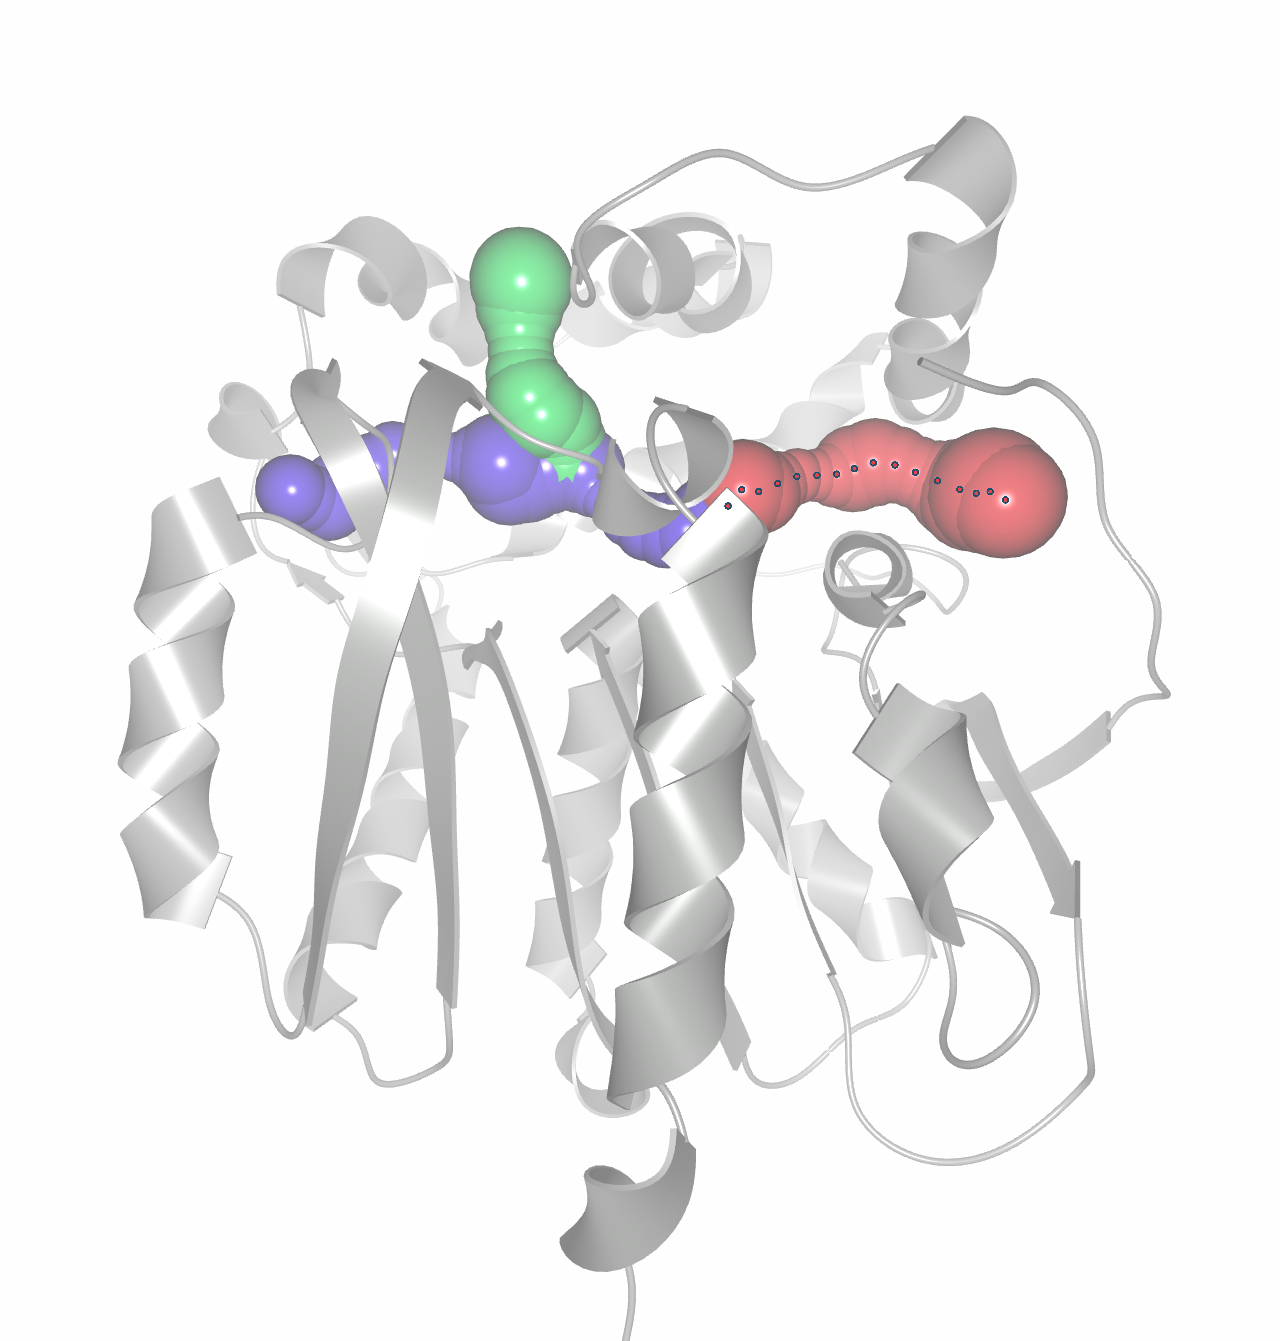
\includegraphics[width=0.3\textwidth]{fig/t05proteintunnels} &
%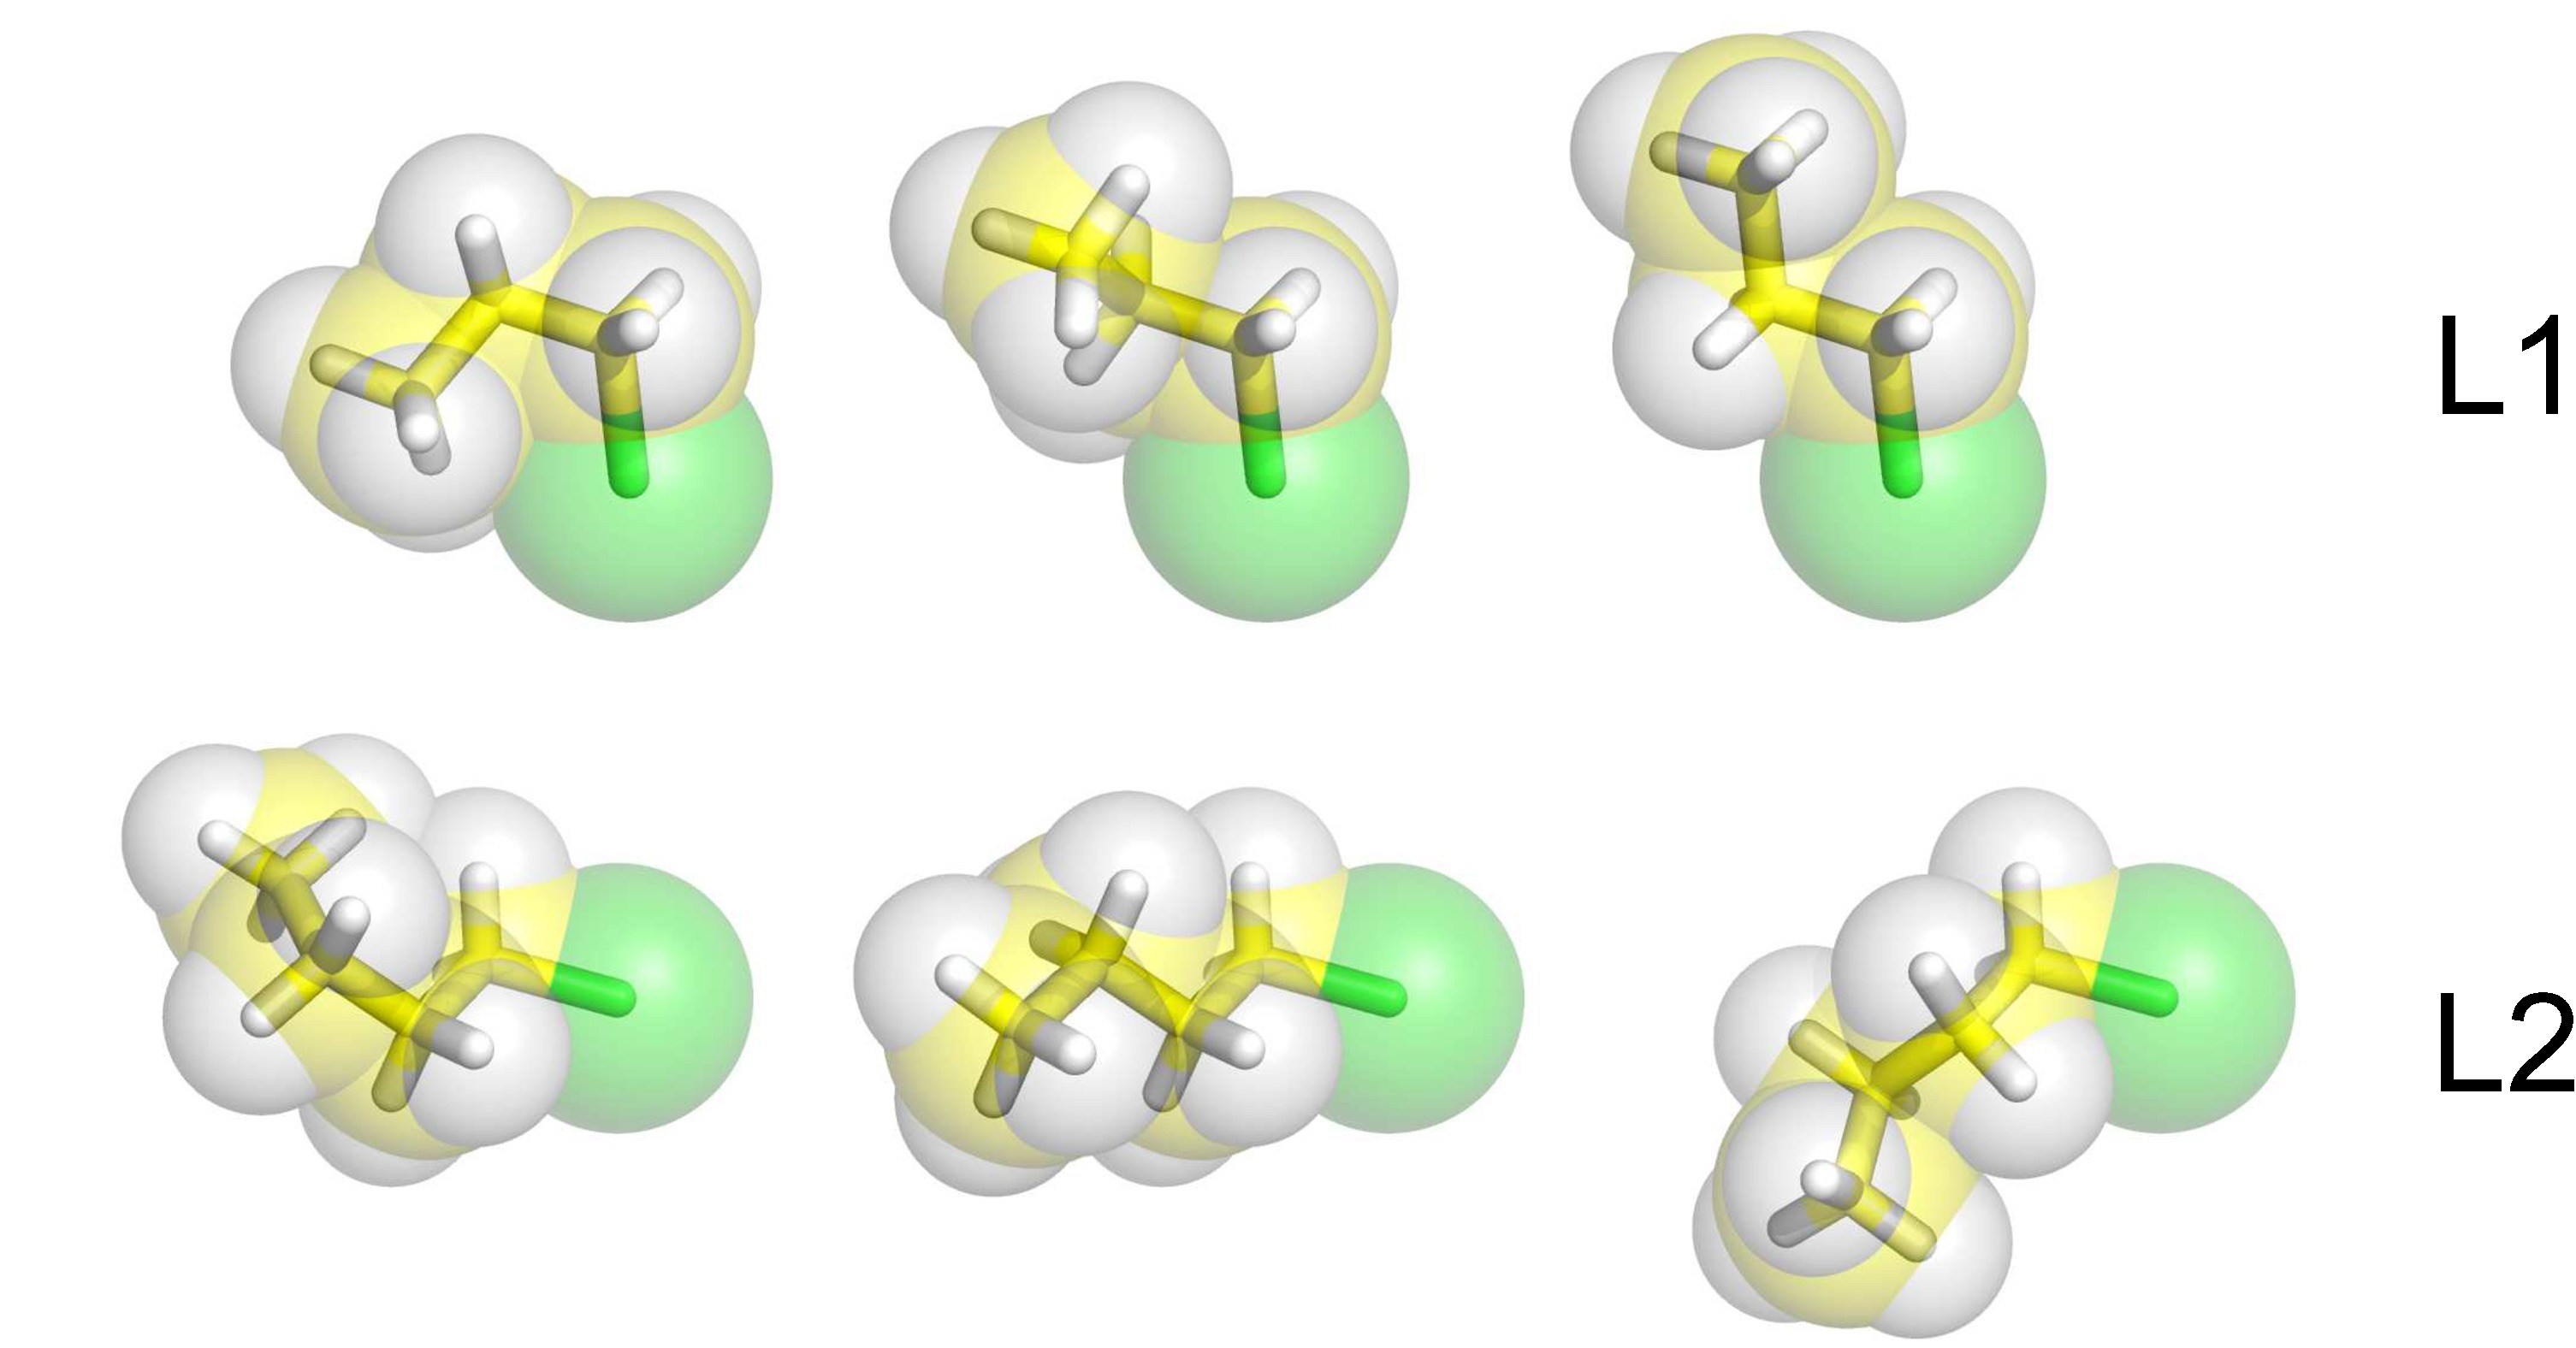
\includegraphics[width=0.45\textwidth]{fig/ligAll}  \\
%(a) & (b)                        
%\end{tabular}                       
%\caption{\label{fig::tunnel}
%    (a) The protein 1CQW visualized using the cartoon representation (gray) with 
%        three tunnels (red, green, blue) detected by CAVER 3.0.
%        The first tunnel is depicted red.
%%        its highest ranked tunnel (green) which was detected using CAVER 3.0.
%    (b) Examples of three conformations of $\LA$ (top) and $\LB$ (bottom)
%}
%\end{figure}
%

\subsection{Influence of the Conformation Selection}

The aim of this experiment was to verify the procedure to select feasible ligand conformations from an available pool of conformations.
Models  of the ligands in Mol2 formats were converted to param files~\cite{meiler2006rosettaligand} containing the topology, rotatable bonds, atom types and partial charges. 
The pool of conformations $\L$ was created by rotation of all rotatable bonds with 30$^\circ$ step using Rosetta3.
The energy cut-off for individual conformations was set to 0.075. %(-rot_ensemble_ecutoff 0.075) 
Two strategies to select a subset from the $\L$ conformations were tested: 
the strategy described in Sec.~\ref{sec::strat} (denoted `S') and the strategy that prefers smaller conformations (denoted `P').
The `P' method selects such conformations where the deviations of the atomic distance from the geometric center are the lowest, which leads 
to the selection of packed conformations.
The strategies were tested using the ligand DCP (Dichloropropanol), for which $1300$ conformations were created, and for the ligand
m040 (1,5-Dichloropentane) with $7560$ conformations.

The traversability rates are shown in Tab.~\ref{tab::selection}, where the subscript of each ligand's 
name shows the number of the selected conformations (5 or 50) and the used method (S or P).
The number after the slash in the ligand's name denotes the number of atoms of the ligand.
In the case of both tested ligands and 50 selected conformations, the `S' strategy leads to a higher traversability rate than the `P' strategy.
For the DCP ligand, higher traversability rate was achieved when 50 conformations were selected.
This experiment shows that selecting 50 conformations using the `S' strategy (Sec.~\ref{sec::strat}) leads to better results
than using a less number of conformations or when preferring the packed conformations.

\begin{table}[ht]
\centering
\caption{\label{tab::selection}
    \small
    The influence of the conformation selection method on the traversability rates in the first (main) tunnel.
    The number after~`$/$' denotes the number of atoms.
    The protein has 4650 atoms. 
    The rate is shown in [\%].
}
\small
\renewcommand{\tabcolsep}{4.3pt}
{\scriptsize
\renewcommand{\arraystretch}{0.7}
\input graphSelNew.tex
}
\end{table}


\subsection{Traversability of Ligands}

Based on the results of the previous experiment, 50 conformations using the `S' strategy were selected for ligands 
m037t (1,2-Dichloroethane), m038t (1,3-Dichloropropane), m056 (2-Chlorobutane), and m080 (Trichloropropane).

    %and Rosetta database 3.2.1 was used during the conformers generation. 
%\cite{meiler2006rosettaligand}
%All substrates were prepared by XXXXXX program and saved in mol2 file. Mol2 formats were converted to param files [1] containing the topology, rotatable bonds, atom types and partial charges by molfile_to_params.py script supplemented in Rosetta Scripts [2]. 
%Rotamer library was created by rotation of all rotatable bonds with 30$^{\circ}$ step. 
%The energy cut-off for individual conformations was set to 0.075. % (-rot_ensemble_ecutoff 0.075) 
%and Rosetta database 3.2.1 was used during the conformers generation.
%Conformations passing the energy criteria were output as multi-pdb file.

\begin{table}[bt]
\centering
\caption{\label{tab::main}
    \small
    Traversability rate [\%] over 100 frames for ligands with 50 conformations. 
    The number after '$/$' denotes the number of atoms.
    The protein has 4650 atoms.
    The rate is shown in [\%].
}
\small
\renewcommand{\tabcolsep}{2pt}
{
\scriptsize
\renewcommand{\arraystretch}{0.7}
\input graphNew.tex
}
\end{table}


The traversability rate is shown in Tab.~\ref{tab::main}. 
The table shows the traversability rate only for the main tunnel, as no trajectory was found in the side tunnel for most of the tested ligands.
The only exception is the ligand m037t, which was the smallest tested one (with 8 atoms), and therefore it could fit even inside the side tunnel.
The traversability rate is higher for the most scaled-down ligands ($\smin=0.5$) and it decreases with the increasing scale.
For the ligand DCP, trajectories were detected in 18~\% of frames for scale $\smin=0.8$ and the traversability of this ligand
to the active site was approved by a separate MD simulation~\cite{marques2017catalytic}.
%For the scale $\smin=0.8$, the most traversable frames were detected for ligands DCP (18~\%), m037t (45~\%) and m038t (30~\%).
%The traversability of the DCP ligand to active site was approved by a separate MD simulation~\cite{marques2017catalytic}.
Based on the number of success rate, also other ligands (e.g., m037t with traversability rate 45~\% at $\smin$=0.8) seem to be promising.
However, their binding was not approved yet by dedicated MD simulations.


Beside scaling-down the ligand, also the atoms of the protein can be scaled, which is used e.g. in~\cite{cortes2005path}.
The tool~\cite{cortes2005path} uses the scale 0.8 for both the ligand and the protein.
We tested also this case using \RA\ (the column \RD\ in Tab.~\ref{tab::main}).
The results are same as for ligand scale $\smin=0.6$  (except DCP and m040 which can be a result of the randomization).



%The number of conformations (out of 50 available) used in the successfull trajectories are shown in Tab.~\ref{tab::m040c}.
%The observed trajectory of the DCP ligand in the MD simulation followed the main tunnel, as expected.
%Based on the traversability rates with $\smin=0.8$, we expect that at least ligands m037t and m038t can also reach the active site, as
%they have the same (or even larger) traversability rate than the DCP.
%However, this hypothesis has not been approved yet by testing it on MD simulations.



\begin{table}[t]
\caption{\label{fig::m040c}
\small
Examples of elongated/packed conformation for m040 (1,5-Dichloropentane).
The table shows the average number of conformations (out of 50) used in trajectories reaching the active site.
}
\centering
{\footnotesize
\def\arraystretch{0.9}
\begin{tabular}{cc}
\rotatebox{0}{\hskip 5pt Long} \\ 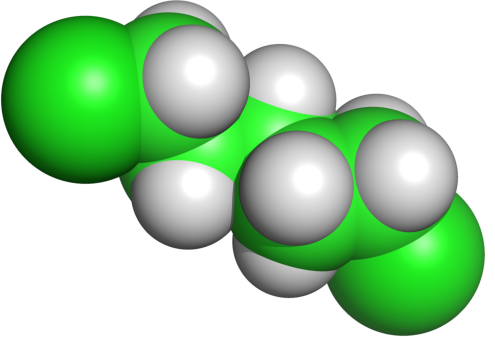
\includegraphics[width=0.1\textwidth]{fig/m040-conf1} \\
\rotatebox{0}{Packed} \\ 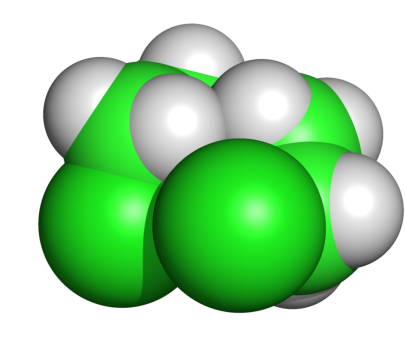
\includegraphics[width=0.078\textwidth]{fig/m040-conf2}
\end{tabular}
}
{\scriptsize
\def\arraystretch{0.9}
\input usedc.tex
}
\end{table}



\section{Discussion and Utilization of the Results}

%originally last two paragraphs in the experiment section, for resubmition, they are moved here to discussion
The proposed \RA\ planner provides higher traversability rate than RRT-Retraction (\RB).
The distances of the configuration trees (measured using the 3D Euclidean metric) to the active site and the runtimes in each frame
are shown in Fig.~\ref{fig::comparison}.
The runtimes of \RB\ are higher than runtimes of \RA and the std. deviations as well.
The variant \RC\ is faster than \RA\ due to simple evaluation of the metric in the expansion step.
%The runtimes of both algorithms increase in those frames, where the tunnel is not traversable, i.e., where the distance
%to the active site is more than 2~\AA\ (for example, in the frame no. 60).
The utilization of the  atom-based metric (used in \RA) leads to higher traversability rate
in the case of large scales and larger ligands (e.g., m056 with $\smin=0.8$: 15~\% with the metric, but to only 6~\% without it).
%Both \RA\ and \RC\ provided trajectories with the same traversability rate in the case of lower scales ($\smin<0.6$).

%The most time-consuming part of the planners is the collision detection. 
%Although both methods can utilize the same number of collision detection queries in the expansion step, 
%\RB\ is slower than \RA, because  \RA\ expands the tree more closer to the random samples $\qrand$ than \RB.
%This results in a faster exploration of the configuration space and therefore, \RA\ needs less number of iterations to reach the active site.

%The better performance of \RA\ is caused by the proposed atom-based metric, because this distance depends on the actual shape of the ligand and 
%it allows the ligands to retract more towards $\qrand$.
%On the contrary, \RB\ utilizes the single 6D Euclidean weighted metric in the expansion, where the weights are the same for all conformations.
%Depending on these weights, the metric favors samples that differ from $\qrand$ more in the rotation or translation part.
%However, the weights between the rotation/translation parts should depend on the shape of the ligand, which is different in each conformation.
%By using a single set of weights in the 6D Euclidean metric, we implicitly favor either the packed or the longer conformations.

The presented work was motivated by the current needs of biochemists who need to analyze the traversability of selected ligands through selected protein tunnels.
Due to low bottleneck of the tunnels, it is often required to shrink the atomic radii of the ligand, as utilized also in other existing tools.
Finding trajectories for the scaled-down ligands enables to solve the problem with narrow passages, but it can be questionable how biochemically relevant such trajectories~are.

Judging the accessibility of the active site by a ligand based only on the traversability rates may be problematic if the ligand is scaled down too much.
Instead of using a single version of the scaled-down ligand, we only limit the minimal scale used by the planner (the parameter $\smin$) and
the planner prefers to apply the higher scales if possible.
%The expansion step always prefers to expand the tree by a collision-free configuration with the maximal scale.
%that leads to a new collision-free configuration.
The information about the scales used at the trajectory points % (which can be extracted from the configuration tree of the proposed planner) 
brings the biochemists new knowledge about the tunnels, which was impossible to get using the VD-based computations.
The  visualization allows the biochemists to observe those parts of the tunnel where the ligand had to be scaled-down significantly (red parts of trajectories in Fig.~\ref{fig::dcp}), and parts where the ligand could be enlarged again (green parts in Fig.~\ref{fig::dcp}).
According to the results of the motion planing, the DCP needs to shrink down to ca. 75~\% of its size (Fig.~\ref{fig::dcp}, point B).
As both the protein and the ligand mutually influence each other, it is possible that even a narrow part of the tunnel is traversable.
This was observed in the MD simulation of the DCP ligand in the 4E46 protein, which revealed that DCP can pass the main tunnel~\cite{marques2017catalytic}.



{\def\a{0}
\begin{figure}[t]
\centering
%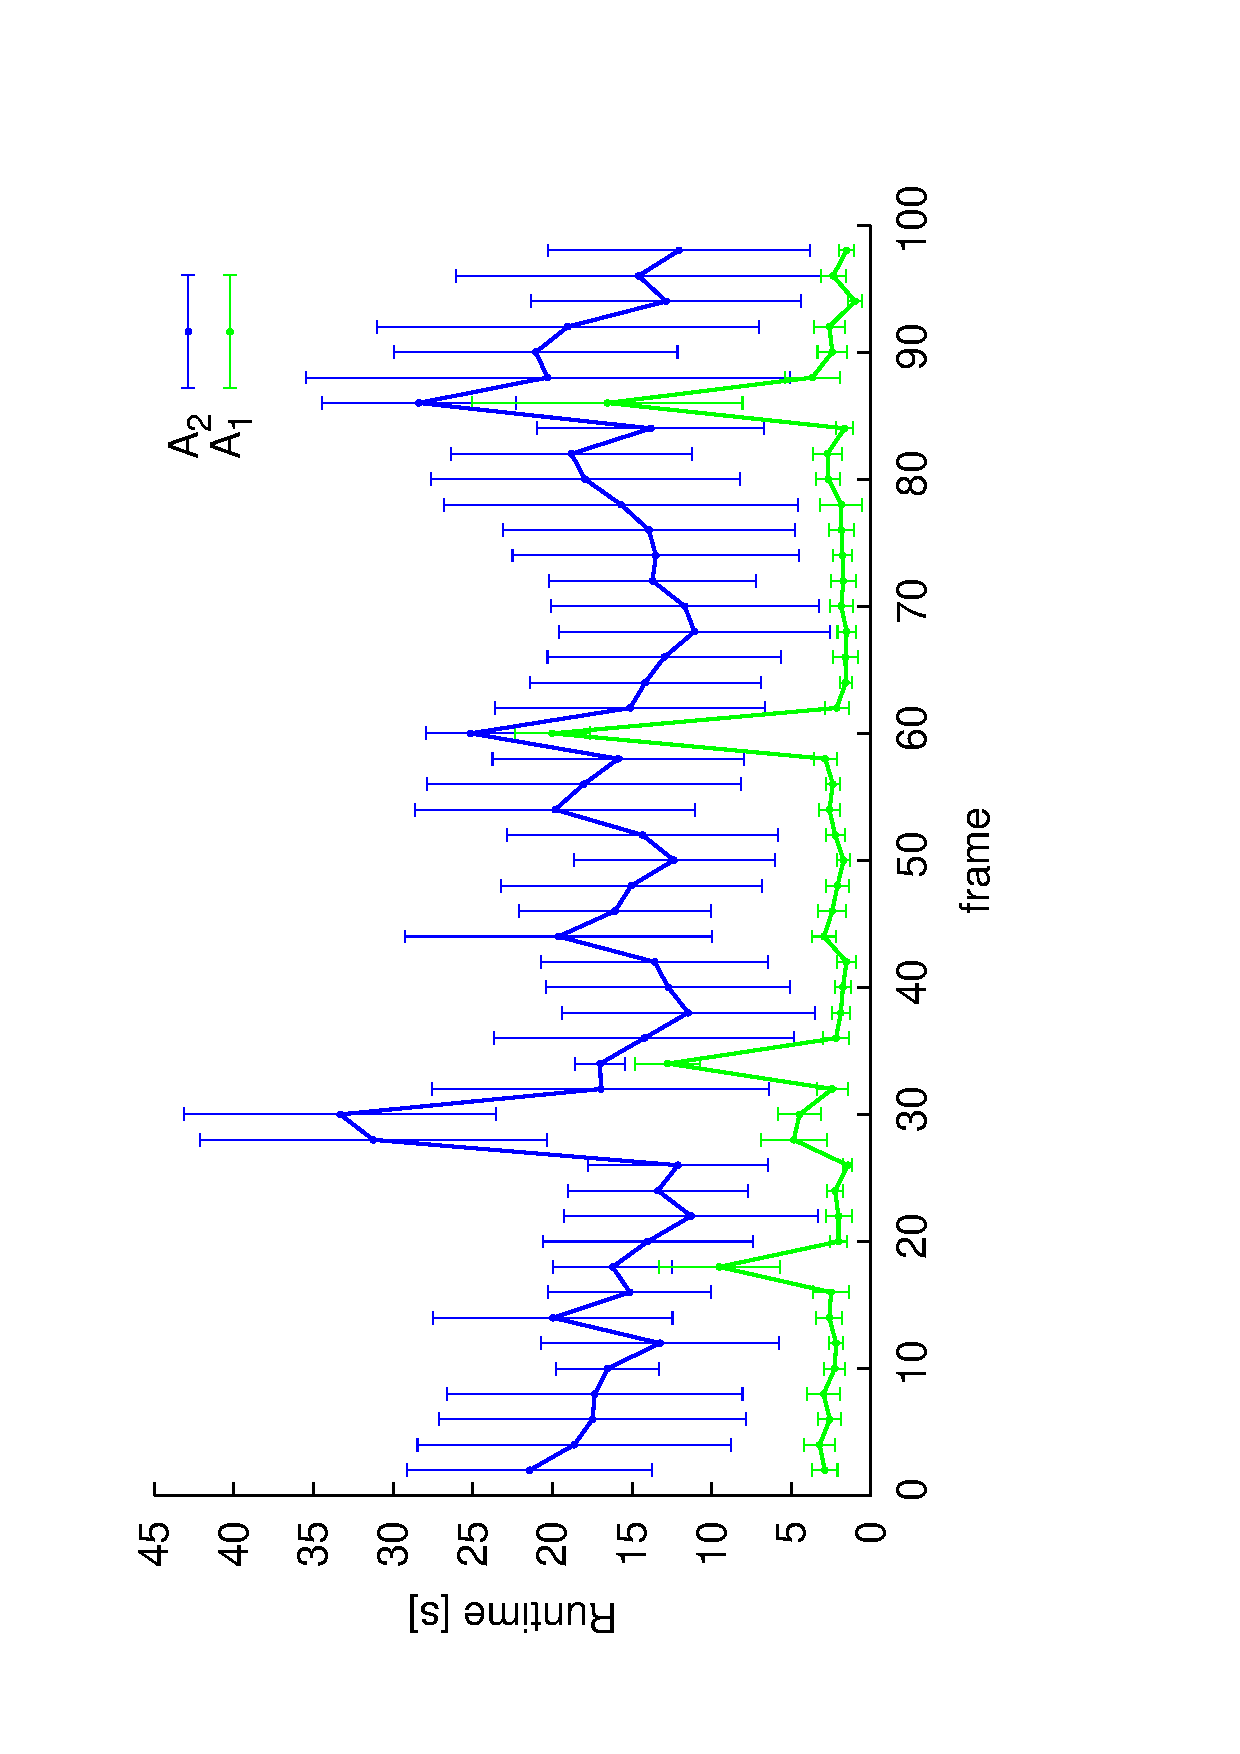
\includegraphics[width=0.17\textwidth,angle=\a]{fig/m037tmins-03tunnel-1rrt_path_time-2}
%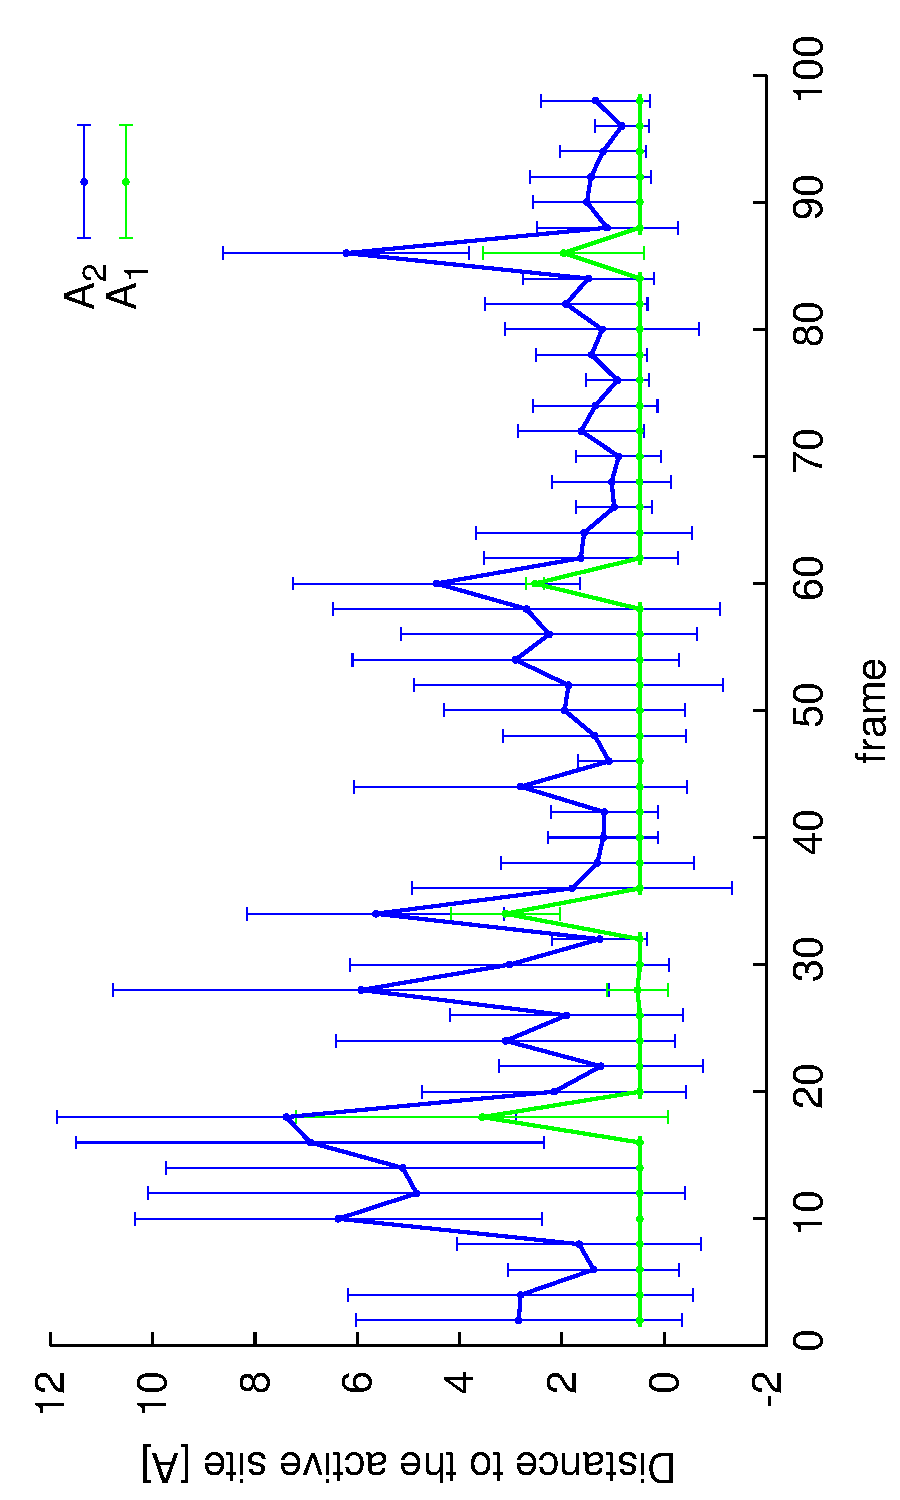
\includegraphics[width=0.17\textwidth,angle=\a]{fig/m037tmins-03tunnel-1trajDistToGoal-2}
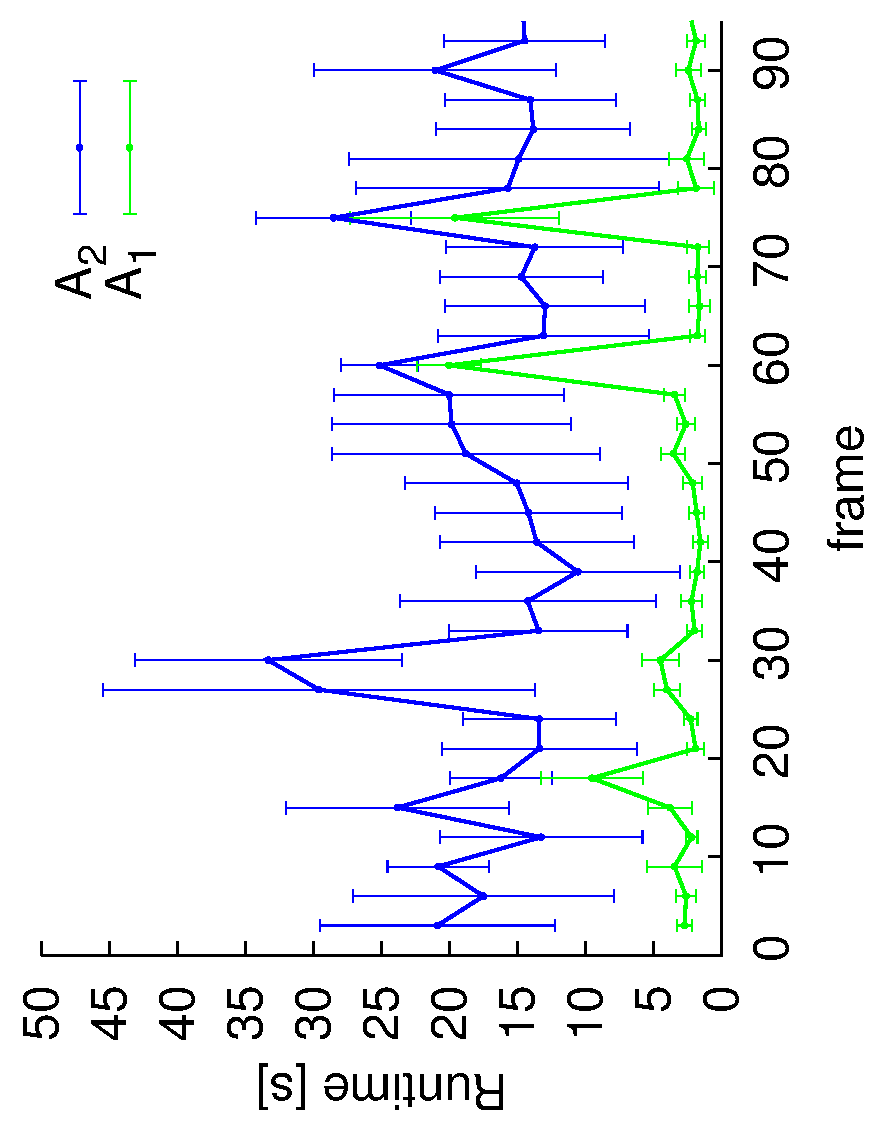
\includegraphics[width=0.22\textwidth,angle=\a]{fig/crop1}
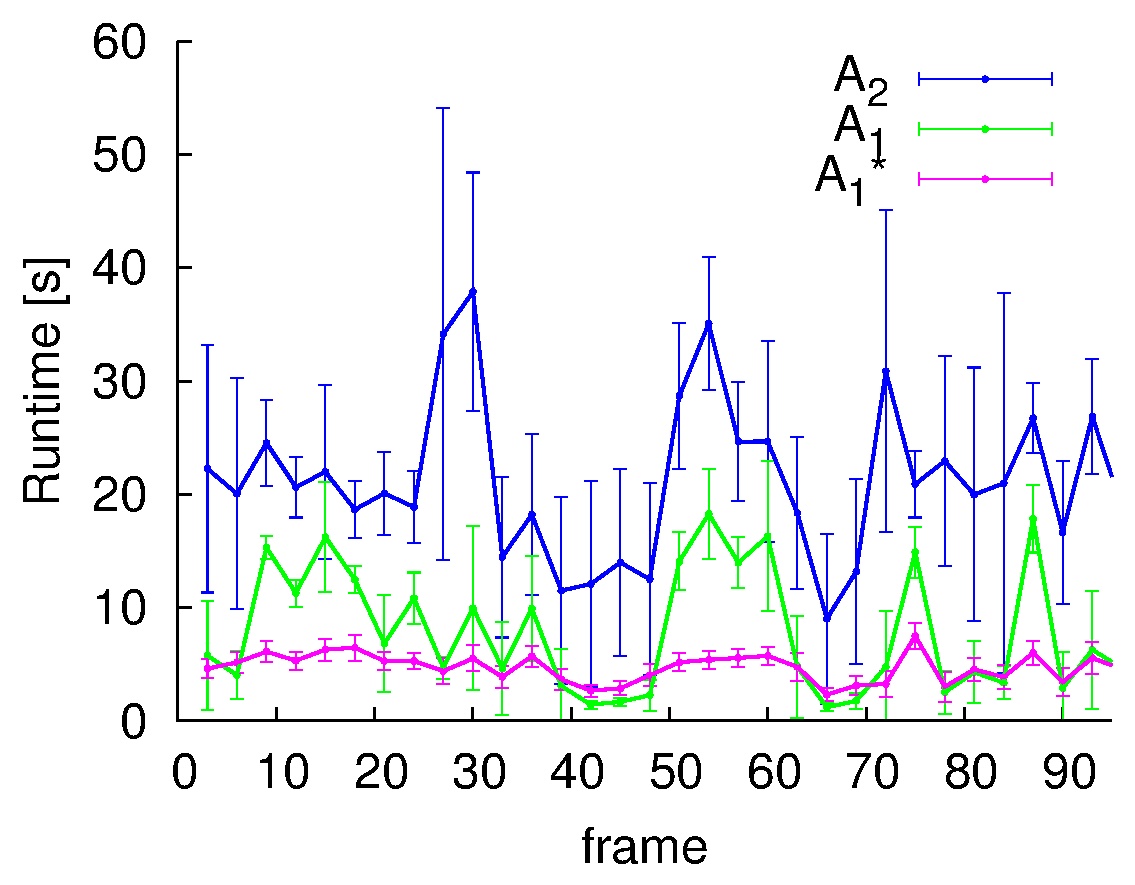
\includegraphics[width=0.22\textwidth,angle=\a]{fig/crop2}
\caption{\label{fig::comparison}
    \small
    Runtimes and the distance to the active site for the m037 ligand at scale 0.7.
    The values are computed from all 200 trials (20 initial configurations $\times$ 10 trials).
    Only each third frame is shown in the graph.
}
\end{figure}
}




\begin{figure}
\centering
\includegraphics[width=0.4\textwidth]{fig/dcp-image1Label}\\
%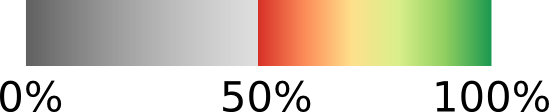
\includegraphics[width=0.2\textwidth]{fig/colormap}
\caption{\label{fig::dcp}
    \small
Visualization of trajectories for the ligand DCP in the two examined tunnels.  
The color of the trajectories corresponds to the scale, that was needed to pass the given part of the tunnel.
The ligand can enter the first tunnel with a high scale (almost 1=100~\%) (A), but then it has to be scaled-down (to $\sim75$~\%) to pass the
next part of the tunnel (B). After this narrow passage, the tunnel is larger again and the ligand can traverse to the narrow passage with
scale $>75$~\% (C).
The second tunnel can also be entered with the high scale (green), but then the narrow part is traversable only with a low scale ($\sim50$~\%) (D). 
For the purpose of the visualization, even more scale-down to 0.3=30~\% was allowed (E) to see how the ligand passed the tunnel.
The ligand can reach the active site only at a very low scale ($\sim0.4=40$~\%) using the side tunnel.
}
\end{figure}


\section{Conclusion}

We presented a novel modification of the RRT planner to compute trajectories of ligands inside selected protein tunnels.
In our solution, we take into account the ligand shape and we model the ligand flexibility using a predefined set of its conformations.
To simulate the real behavior of ligand passing through a tunnel, we enable scaling down the atomic radii of the ligands up to a certain predefined factor.
The planner generates the random samples only along a tunnel computed by Voronoi diagram, and it attempts to expand the configuration
tree using all ligand conformations. 
The expansion prefers atoms with a higher scale, which ensures that the ligand shrinks down only if necessary, i.e., when traversing the narrow parts of the tunnel.
To further boost the exploration of the configuration space, a novel metric suitable for measuring the distances between various ligand shapes is used in the expansion step.
The proposed method has been used to test and evaluate the trajectories of several ligands in a sequence of frames capturing protein dynamics.


\bibliographystyle{plain}
\bibliography{paper}

\end{document}

% ====================================================
% ====================================================
% ====================================================
% ====================================================
% ====================================================
% ====================================================

% ============  unused ideas =========================

%neni treba \cite{cheng01reducing}
%Using a library of predefined conformations has been used also in other tasks, e.g.~\cite{kellogg}.
%This shrinking technique is also used in the MoMa-LigPath tool~\cite{cortes2005path}, which utilizes RRT to find pathways for unbinding a ligand  from a protein.
%It is necessary to use an apporpriated distance metric in the configuration space.
%Generally, it is hard to combine the translational and rotational components in the configuration space.
%In~\cite{zhangRetraction}, the DISP metric~\cite{zhang2008fast}.
%energetic constraints are translated into geometric ones by considering a steric model of the molecules and applying collision detection
%\cite{deAngulo2005biocd}
%First the biredge test is applied to identify regions aeround narrow passages, optimization-based retraction operatoin sleectively only at those regions selective rrt~\cite{lee2012srrrt}
%Free-space dilation is an effective aproach for narrow passage sampling~\cite{hsu06multilevel}. 
%It is necessary to define proper method for dilating and determin the amount of dilation.
%\cite{saha2005finding}
%DISP metric \cite{zhang2008fast}

